\documentclass[12pt]{article}
\usepackage{fancyhdr} % 用于自定义页眉页脚
\usepackage{listings} % 用于代码高亮
\usepackage{xcolor} % 用于定义颜色
\usepackage{fontspec} % 用于设置字体 (需要XeLaTeX或LuaLaTeX)
\usepackage{graphicx} % 用于插入图片
\usepackage{float} % 用于强制图片位置
\usepackage{geometry} % 用于设置页面边距
\usepackage{subcaption}

\geometry{a4paper, margin=0.9in} % 设置A4纸大小和0.9英寸边距

% 设置图片路径
\graphicspath{{./fig/}} % 假设图片存放在images文件夹中

% 定义VS Code风格的颜色
\definecolor{vscode-bg}{RGB}{30,30,30}
\definecolor{vscode-string}{RGB}{206,145,120}
\definecolor{vscode-keyword}{RGB}{86,156,214}
\definecolor{vscode-comment}{RGB}{106,153,85}
\definecolor{vscode-number}{RGB}{181,206,168}
\definecolor{vscode-function}{RGB}{220,220,170}

% 设置代码块字体(Fira Code或Consolas或Monaco)
\setmonofont{Consolas}[Scale=0.9]

% 配置listings样式
\lstdefinestyle{vscode}{
    backgroundcolor=\color{vscode-bg},
    commentstyle=\color{vscode-comment},
    keywordstyle=\color{vscode-keyword}\bfseries,
    numberstyle=\tiny\color{white},
    stringstyle=\color{vscode-string},
    basicstyle=\ttfamily\footnotesize\color{white},
    breakatwhitespace=false,
    breaklines=true,
    captionpos=b,
    keepspaces=true,
    numbers=left,
    numbersep=5pt,
    showspaces=false,
    showstringspaces=false,
    showtabs=false,
    tabsize=2,
    frame=single,
    frameround=tttt,
    rulecolor=\color{gray!30}
}

% 设置默认代码样式
\lstset{style=vscode}

\title{GalPHOS Project Report}
\author{\textbf{Group 16}: Hengxu Wu, Kairui Li, Yangyi Xiong}
\date{}

% 设置页面样式
\pagestyle{fancy}
\fancyhf{} % 清除所有页眉页脚
\fancyhead[L]{\leftmark} % 左上方显示section
\fancyhead[R]{\rightmark} % 右上方显示subsection
\fancyfoot[C]{\thepage} % 页脚中央显示页码

% 重新定义section和subsection的标记格式
\renewcommand{\sectionmark}[1]{\markboth{#1}{}}
\renewcommand{\subsectionmark}[1]{\markright{#1}}

\begin{document}

\makeatletter % change default title style
\renewcommand*\maketitle{%
    \begin{center}% 
        {\LARGE \@title \par} %
        \vskip 1em%
        {\large
        \lineskip .75em%
        \begin{tabular}[t]{c}%
            \@author
        \end{tabular}\par}%
        \thispagestyle{empty} %
    \end{center}%
    \setcounter{footnote}{0}%
}
\makeatother

\maketitle

\section{Introduction}
\subsection{Project Overview}
% 简单介绍项目的内容和情况

GalPHOS (Galaxy Physics Online System) is a physical competition event management system based on the web platform, covering a variety of functions including event registration, exam management, and score statistics. The system is designed to provide an efficient and convenient management platform for physics competitions, supporting a variety of user roles, including administrators, students, coaches and graders.

Our system architecture and functions are based on the life cycle design of a competition, including five stages: registration, pre-match preparation, answer submission, post-match marking, result statistics and archives. The figure below illustrates the workflow of the system.
\begin{figure}[H]
    \centering
    \includegraphics[width=\textwidth]{Fig1.png}
    \caption{GalPHOS System Workflow}
    \label{fig:workflow}
\end{figure}

\subsection{Our Work}
% 介绍小组成员的工作内容和分工

Our group consists of three members: Hengxu Wu, Kairui Li, and Yangyi Xiong. The leader of the group is Hengxu Wu. Each member has contributed to different aspects of the project:
\begin{itemize}
    \item Hengxu Wu: Responsible for project design, development documents, and front-end development.
    \item Kairui Li: Responsible for project design, development documents, and part of the back-end development, including Exam Management Service, File Storage Service, Region Management Service and Submission Service.
    \item Yangyi Xiong: Responsible project design, development documents, and part of the back-end development, including GradingService, ScoreStatisticsService, SystemConfigService, UserAuthService and UserManagementService.
\end{itemize}

\section{System Architecture}
% \subsection{Architecture Overview}
% 描述系统的整体架构和设计思路,包括前端和后端的分离
\subsection{Frontend Design}
% 介绍前端的设计和实现(类型这一块)
\subsection{Backend Design}

\subsubsection{System Overview}

The GalPHOS backend is a microservices-based platform engineered to deliver reliable, scalable, and maintainable operations for physics olympiad competitions. 

The architecture consists of 9 specialized microservices: Exam Management Service, File Storage Service, Region Management Service, Submission Service, Grading Service, Score Statistics Service, System Config Service, User Authentication Service and User Management Service. All of them are designed with type-safe domain modeling using Scala's advanced type system. Every component follows functional programming principles, leveraging algebraic data types (ADTs), effect types, and compile-time guarantees to ensure system reliability and maintainability. And all side effects are captured in the type system using Cats Effect's `IO' monad, making impure operations explicit and composable.

As for APIs, the API architecture adheres to modern RESTful design principles. All API endpoints are defined using HTTP4s with strong typing that ensures request/response contracts are validated at compile time. 

For data structures, the backend employs a sdata architecture with microservice-specific database isolation. Each service maintains its own PostgreSQL database, ensuring data autonomy and service independence.

The type-safe architecture ensures that the GalPHOS system maintains data integrity, prevents runtime errors, and provides clear contracts between all system components, from frontend interactions to database operations.

\subsubsection{Microservices Architecture Overview}

Consistent with what was mentioned earlier, the system consists of 9 specialized microservices, each handling distinct business domains. And the figure below illustrates the overall architecture of the GalPHOS system, showcasing the microservices and their interactions.

\begin{figure}[H]
    \centering
    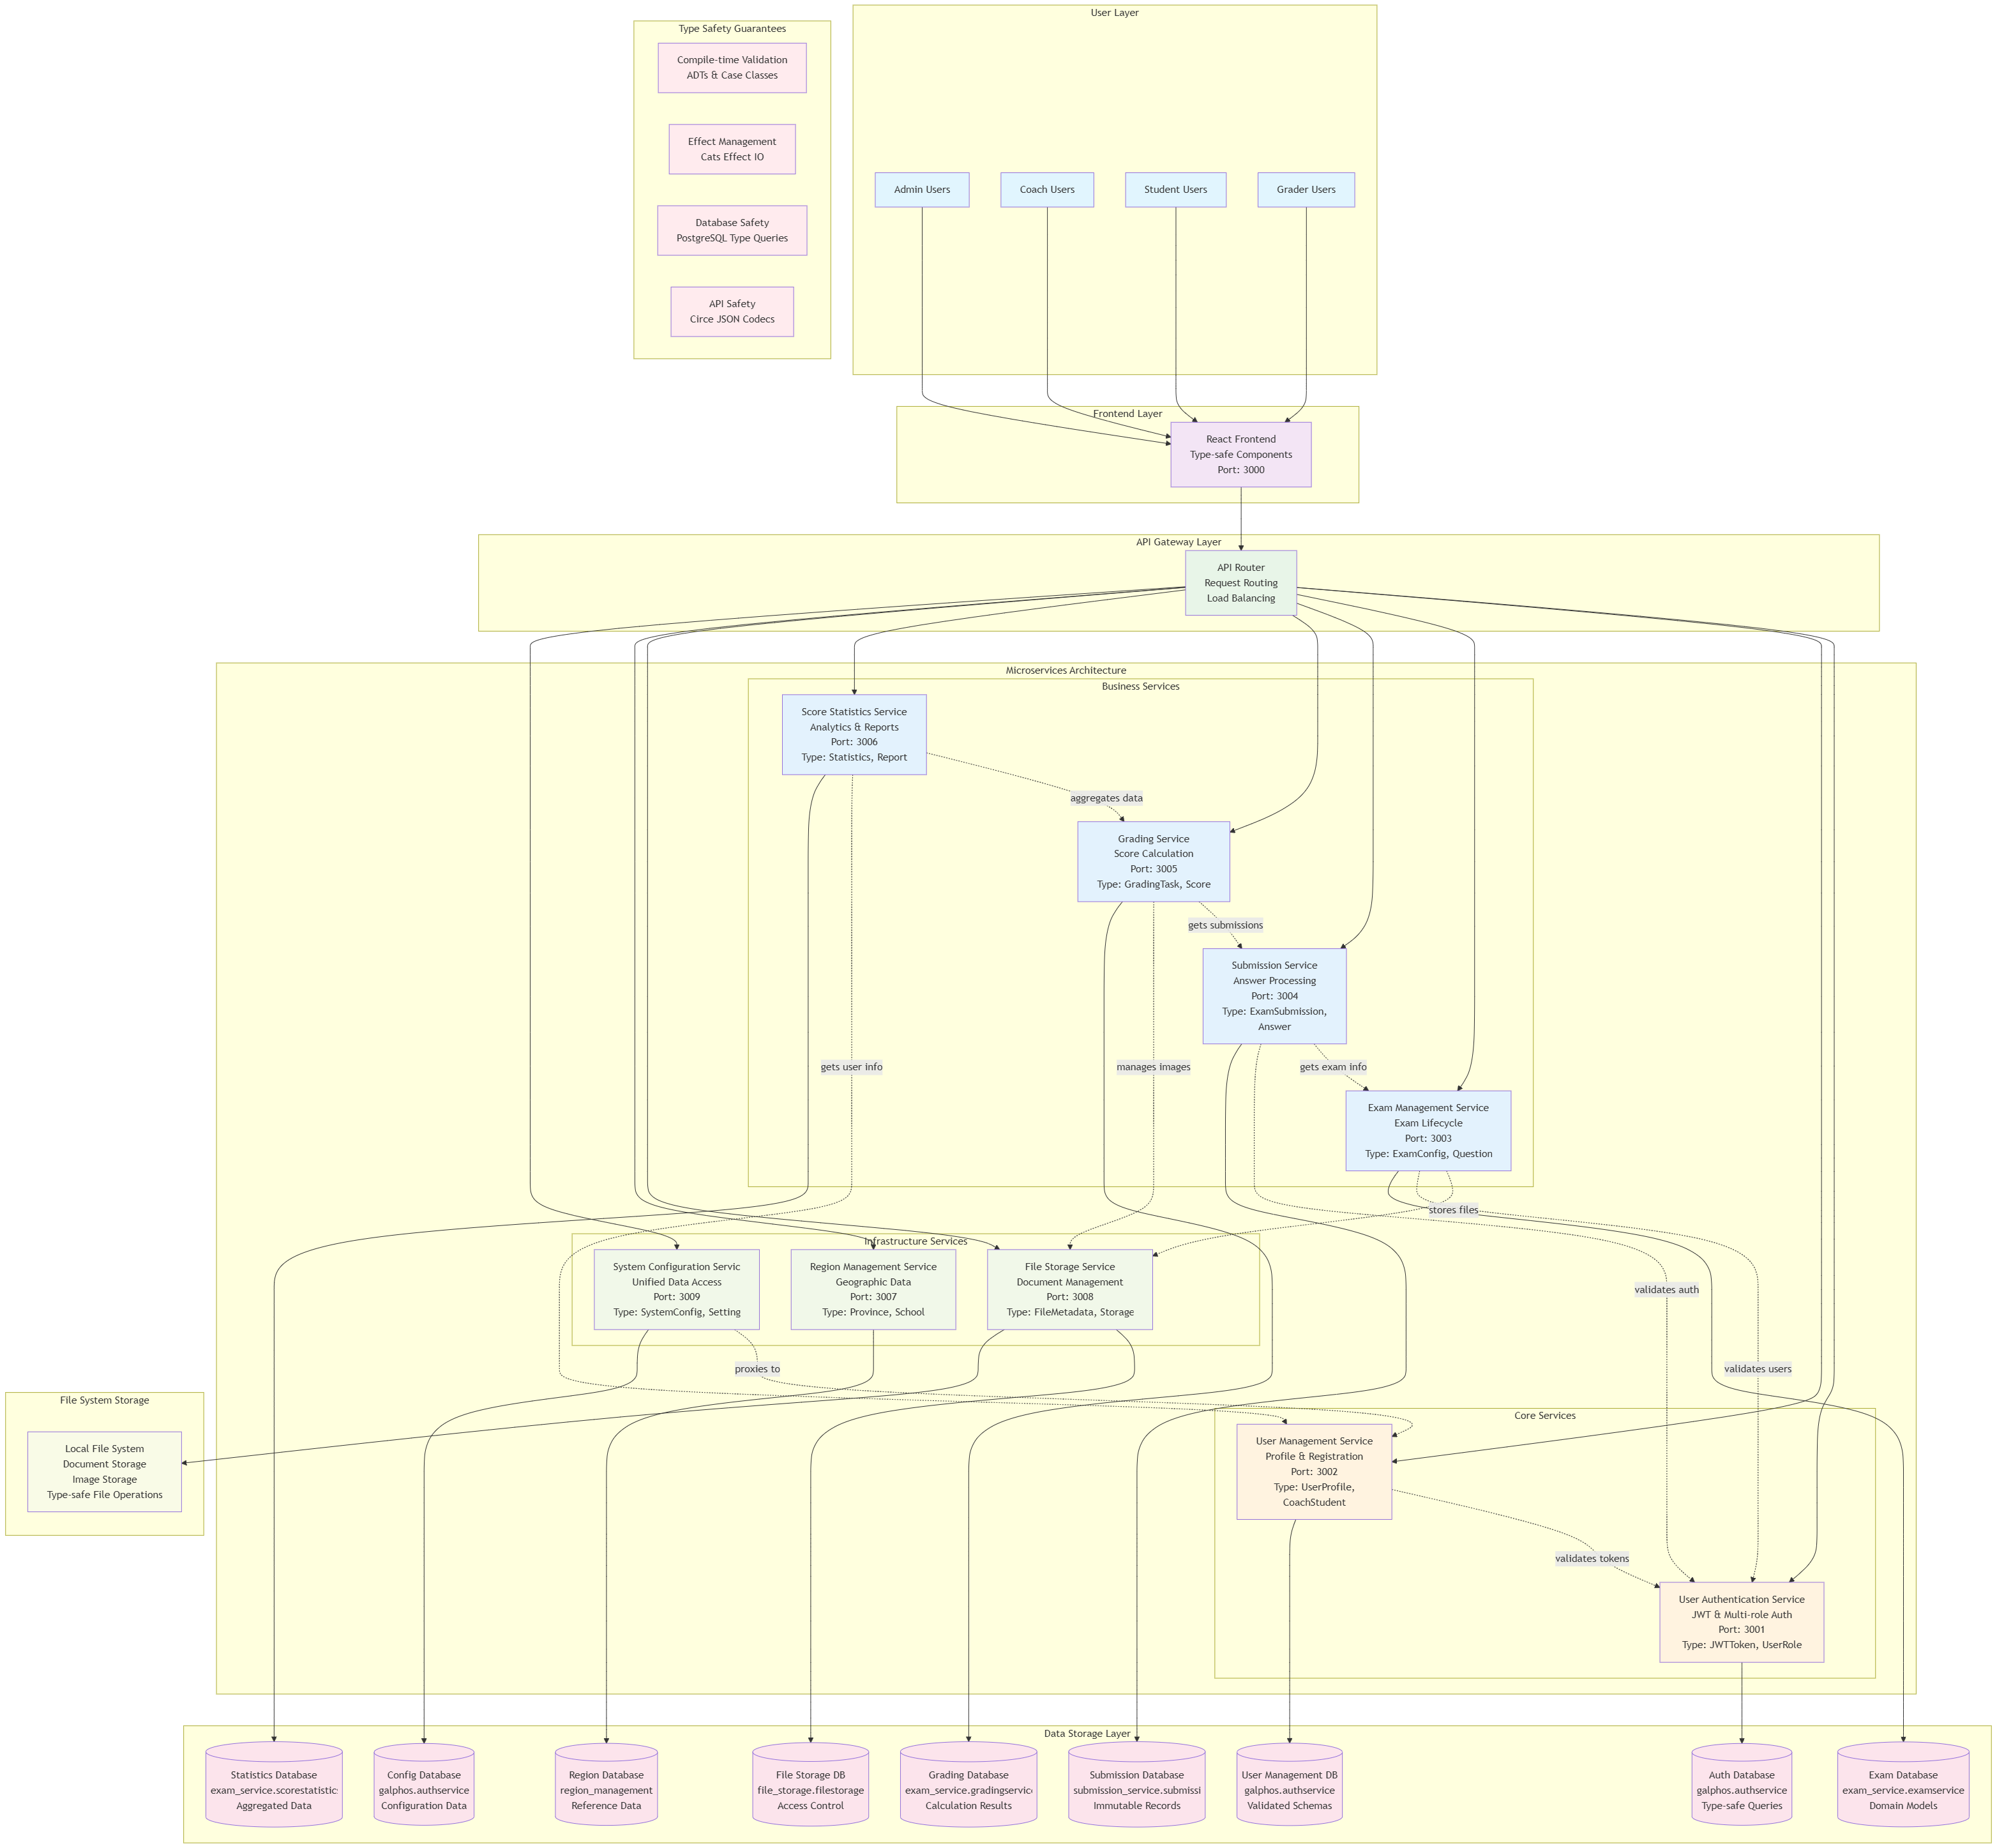
\includegraphics[width=\textwidth]{Fig2.png}
    \caption{Microservices Architecture}
    \label{fig:ArchitectureOverview}
\end{figure}

\subsubsection{Core Components}

Now, let me introduce each of the 9 microservices one by one.

\paragraph{User Authentication Service} (on Port 3001) is responsible for handling all authentication, authorization, and session management operations. It provides APIs for user login and registration with role-based authentication, JWT token generation and validation, password security using SHA-256 with salt values, and cross-service authentication validation for inter-service communication. Some examples of type-safe components:

\begin{lstlisting}[language=Scala]
case class LoginRequest( role: String, username: String, password: String )

enum UserStatus(val value: String):
  case Pending extends UserStatus("PENDING")
  case Active extends UserStatus("ACTIVE")
  case Disabled extends UserStatus("DISABLED")
\end{lstlisting}

\paragraph{User Management Service} (on Port 3002) is responsible for comprehensive user lifecycle management, user information maintenance, coach-student relationship management, and region administration operations. It provides APIs for user approval and review processes with pending user management and batch approval operations, user status lifecycle management, coach-student relationship establishment and maintenance with statistics tracking, region change request processing for students and coaches with administrative approval workflows, and administrative user management. Some examples of type-safe components:

\begin{lstlisting}[language=Scala]
case class CoachStudentRelationship( id: String, coachId: String, coachUsername: String, coachName: Option[String], studentId: String, studentUsername: String, studentName: Option[String], createdAt: LocalDateTime )

case class RegionChangeRequest( province: String, school: String, reason: String )
\end{lstlisting}

\paragraph{Exam Management Service} (on Port 3003) is responsible for complete exam lifecycle management including creation, modification, publication, status tracking, and coordination with other services throughout the examination process. It provides APIs for exam CRUD operations with role-based access control, question score configuration and management, file upload integration supporting multiple file types (question papers, answer keys, answer sheets), exam status management with automated transitions, submission coordination with external services, and comprehensive exam statistics and monitoring capabilities. Some examples of type-safe components:

\begin{lstlisting}[language=Scala]
case class Exam( id: String, title: String, description: String, startTime: LocalDateTime, endTime: LocalDateTime, status: ExamStatus, createdAt: LocalDateTime, updatedAt: LocalDateTime, duration: Option[Int] = None, questionFile: Option[ExamFile] = None, answerFile: Option[ExamFile] = None, answerSheetFile: Option[ExamFile] = None, createdBy: String, participants: List[String] = List.empty, totalQuestions: Option[Int] = None, maxScore: Option[Double] = None, totalScore: Option[Double] = None, subject: Option[String] = None, instructions: Option[String] = None )

case class CreateExamRequest( title: String, description: String, startTime: LocalDateTime, endTime: LocalDateTime, totalQuestions: Int, duration: Int, status: ExamStatus = ExamStatus.Draft, totalScore: Option[Double] = None, questions: Option[List[CreateExamQuestionRequest]] = None )
\end{lstlisting}

\paragraph{Submission Service} (on Port 3004) is responsible for managing exam answer submissions, supporting both independent student direct submissions and coach proxy submissions for non-independent students. It provides APIs for student answer submission, file upload management and submission status tracking. The corresponding database has two main tables: `submissions' table for storing exam submission records with metadata, and `answers' table for storing individual question answers with image URLs, scores, and grading details. Some examples of type-safe components:

\begin{lstlisting}[language=Scala]
enum SubmissionStatus(val value: String) {
  case Submitted extends SubmissionStatus("submitted")
  case Grading extends SubmissionStatus("grading")
  case Graded extends SubmissionStatus("graded")
}

case class ExamSubmission( id: String, examId: String, studentId: String, studentUsername: String, studentName: Option[String] = None, answers: List[ExamAnswer], submittedAt: LocalDateTime, status: SubmissionStatus, totalScore: Option[Double] = None, maxScore: Option[Double] = None, gradedAt: Option[LocalDateTime] = None, gradedBy: Option[String] = None, feedback: Option[String] = None, submittedBy: Option[String] = None )
\end{lstlisting}

\paragraph{Grading Service} (on Port 3005) is responsible for managing the entire grading workflow for online examinations, including task assignment, score management, and grading progress tracking. It provides APIs for administrators to create and assign grading tasks, monitor grading progress, configure question scores, and for graders to perform actual grading work. The corresponding database has tables to manage individual grading assignments, store question-specific scoring configurations, maintaine grading audit trails, and store submission images. Some examples of type-safe components:

\begin{lstlisting}[language=Scala]
case class TaskAssignmentRequest( examId: String, graderId: String, questionIds: List[String] )

case class GradingProgress( examId: String, totalTasks: Int, completedTasks: Int, inProgressTasks: Int, pendingTasks: Int, completionPercentage: BigDecimal )
\end{lstlisting}

\paragraph{Score Statistics Service} (on Port 3006) is responsible for handling student score calculations, statistical analysis and ranking generation. It provides APIs for student score viewing and ranking retrieval, coach grade management and student performance monitoring and grader statistics tracking. The corresponding database has tables to store individual student exam results with ranking and percentile information, individual student performance tracking over time, coach-level performance metrics and so on. Some examples of type-safe components:

\begin{lstlisting}[language=Scala]
case class ExamScore( id: Option[Int] = None, examId: Int, studentId: Int, totalScore: Double, questionScores: Map[String, Double] = Map.empty, rankPosition: Int = 0, percentile: Double = 0.0, createdAt: Option[LocalDateTime] = None, updatedAt: Option[LocalDateTime] = None )

case class StudentStatistics( id: Option[Int] = None, studentId: Int, totalExams: Int, averageScore: Double, bestScore: Double, worstScore: Double, improvementTrend: Double, strongSubjects: List[String] = List.empty, weakSubjects: List[String] = List.empty, createdAt: Option[LocalDateTime] = None, updatedAt: Option[LocalDateTime] = None )
\end{lstlisting}

\paragraph{Region Management Service} (on Port 3007) is responsible for managing geographical regions and handling region change requests from students and coaches. It provides APIs for CRUD operations on provinces and schools. The service implements role-based access control with different endpoints for administrators, students, and coaches, and includes authentication integration with the User Authentication Service. The corresponding database has three main tables, respectively for storing province information with UUID primary keys, linking provinces with foreign key relationships, and tracking user requests for region changes. Some examples of type-safe components:

\begin{lstlisting}[language=Scala]
case class Province( id: UUID, name: String, createdAt: OffsetDateTime, updatedAt: OffsetDateTime )

case class School( id: UUID, name: String, provinceId: UUID, province: Option[Province] = None, createdAt: OffsetDateTime, updatedAt: OffsetDateTime )
\end{lstlisting}

\paragraph{File Storage Service} (on Port 3008) is responsible for handling all file upload, download, and management operations. It provides APIs for uploading multiple file types including exam files, answer images, documents, and avatars, with role-based access control for different user types (admins, students, coaches, and graders). The corresponding database includes metadata of each files and optimized indexes for efficient querying by exam ID, student ID, category, and upload time. Some examples of type-safe components:

\begin{lstlisting}[language=Scala]
enum FileCategory(val value: String):
  case Avatar extends FileCategory("avatar")
  case AnswerImage extends FileCategory("answer-image")
  case ExamFile extends FileCategory("exam-file")
  case Document extends FileCategory("document")
  case Other extends FileCategory("other")

case class FileRecord( id: String, fileName: String, originalName: String, fileUrl: String, fileSize: Long, mimeType: String, fileType: Option[String] = None, category: Option[String] = None, examId: Option[String] = None, questionNumber: Option[Int] = None, studentId: Option[String] = None, uploadedBy: String, uploadTime: LocalDateTime )
\end{lstlisting}

\paragraph{System Configuration Service} (on Port 3009) is responsible for managing system-wide configurations, administrator accounts, and providing unified data access across all services in the GalPHOS system. It provides APIs for system settings management, administrator account operations, unified user data access through proxy services, version information management, and global system configuration. The corresponding database stores system configurations and administrator data managed through UserAuthService integration. Some examples of type-safe components:

\begin{lstlisting}[language=Scala]
case class SystemConfig( id: Option[Long], configKey: String, configValue: String, description: Option[String], isPublic: Boolean, createdAt: Option[ZonedDateTime], updatedAt: Option[ZonedDateTime] )

case class Admin( id: Option[String], username: String, passwordHash: Option[String], role: String, isSuperAdmin: Boolean, status: Option[String], createdAt: Option[ZonedDateTime], updatedAt: Option[ZonedDateTime], lastLogin: Option[ZonedDateTime] )
\end{lstlisting}

% \subsubsection{Example: The Complete Exam Workflow}
% 
% This example demonstrates the entire exam lifecycle from creation to grading completion, showcasing type-safe inter-service communication and state management.
% 
% \begin{figure}[H]
%     \centering
%     \includegraphics[width=\textwidth]{Fig3.png}
%     \caption{Example: The Complete Exam Workflow}
%     \label{fig:Example}
% \end{figure}

\section{Usage and Features}
\subsection{Administrator}
\subsubsection{Admin Management}
We have a super administrator account initialized along with the system, which has username and password both initialized but can be changed later. All other administrators are added by
the super administrator later, and super admin can manage them by adding, deleting, banning and password reseting.
% \begin{figure}[H]
%     \centering
%     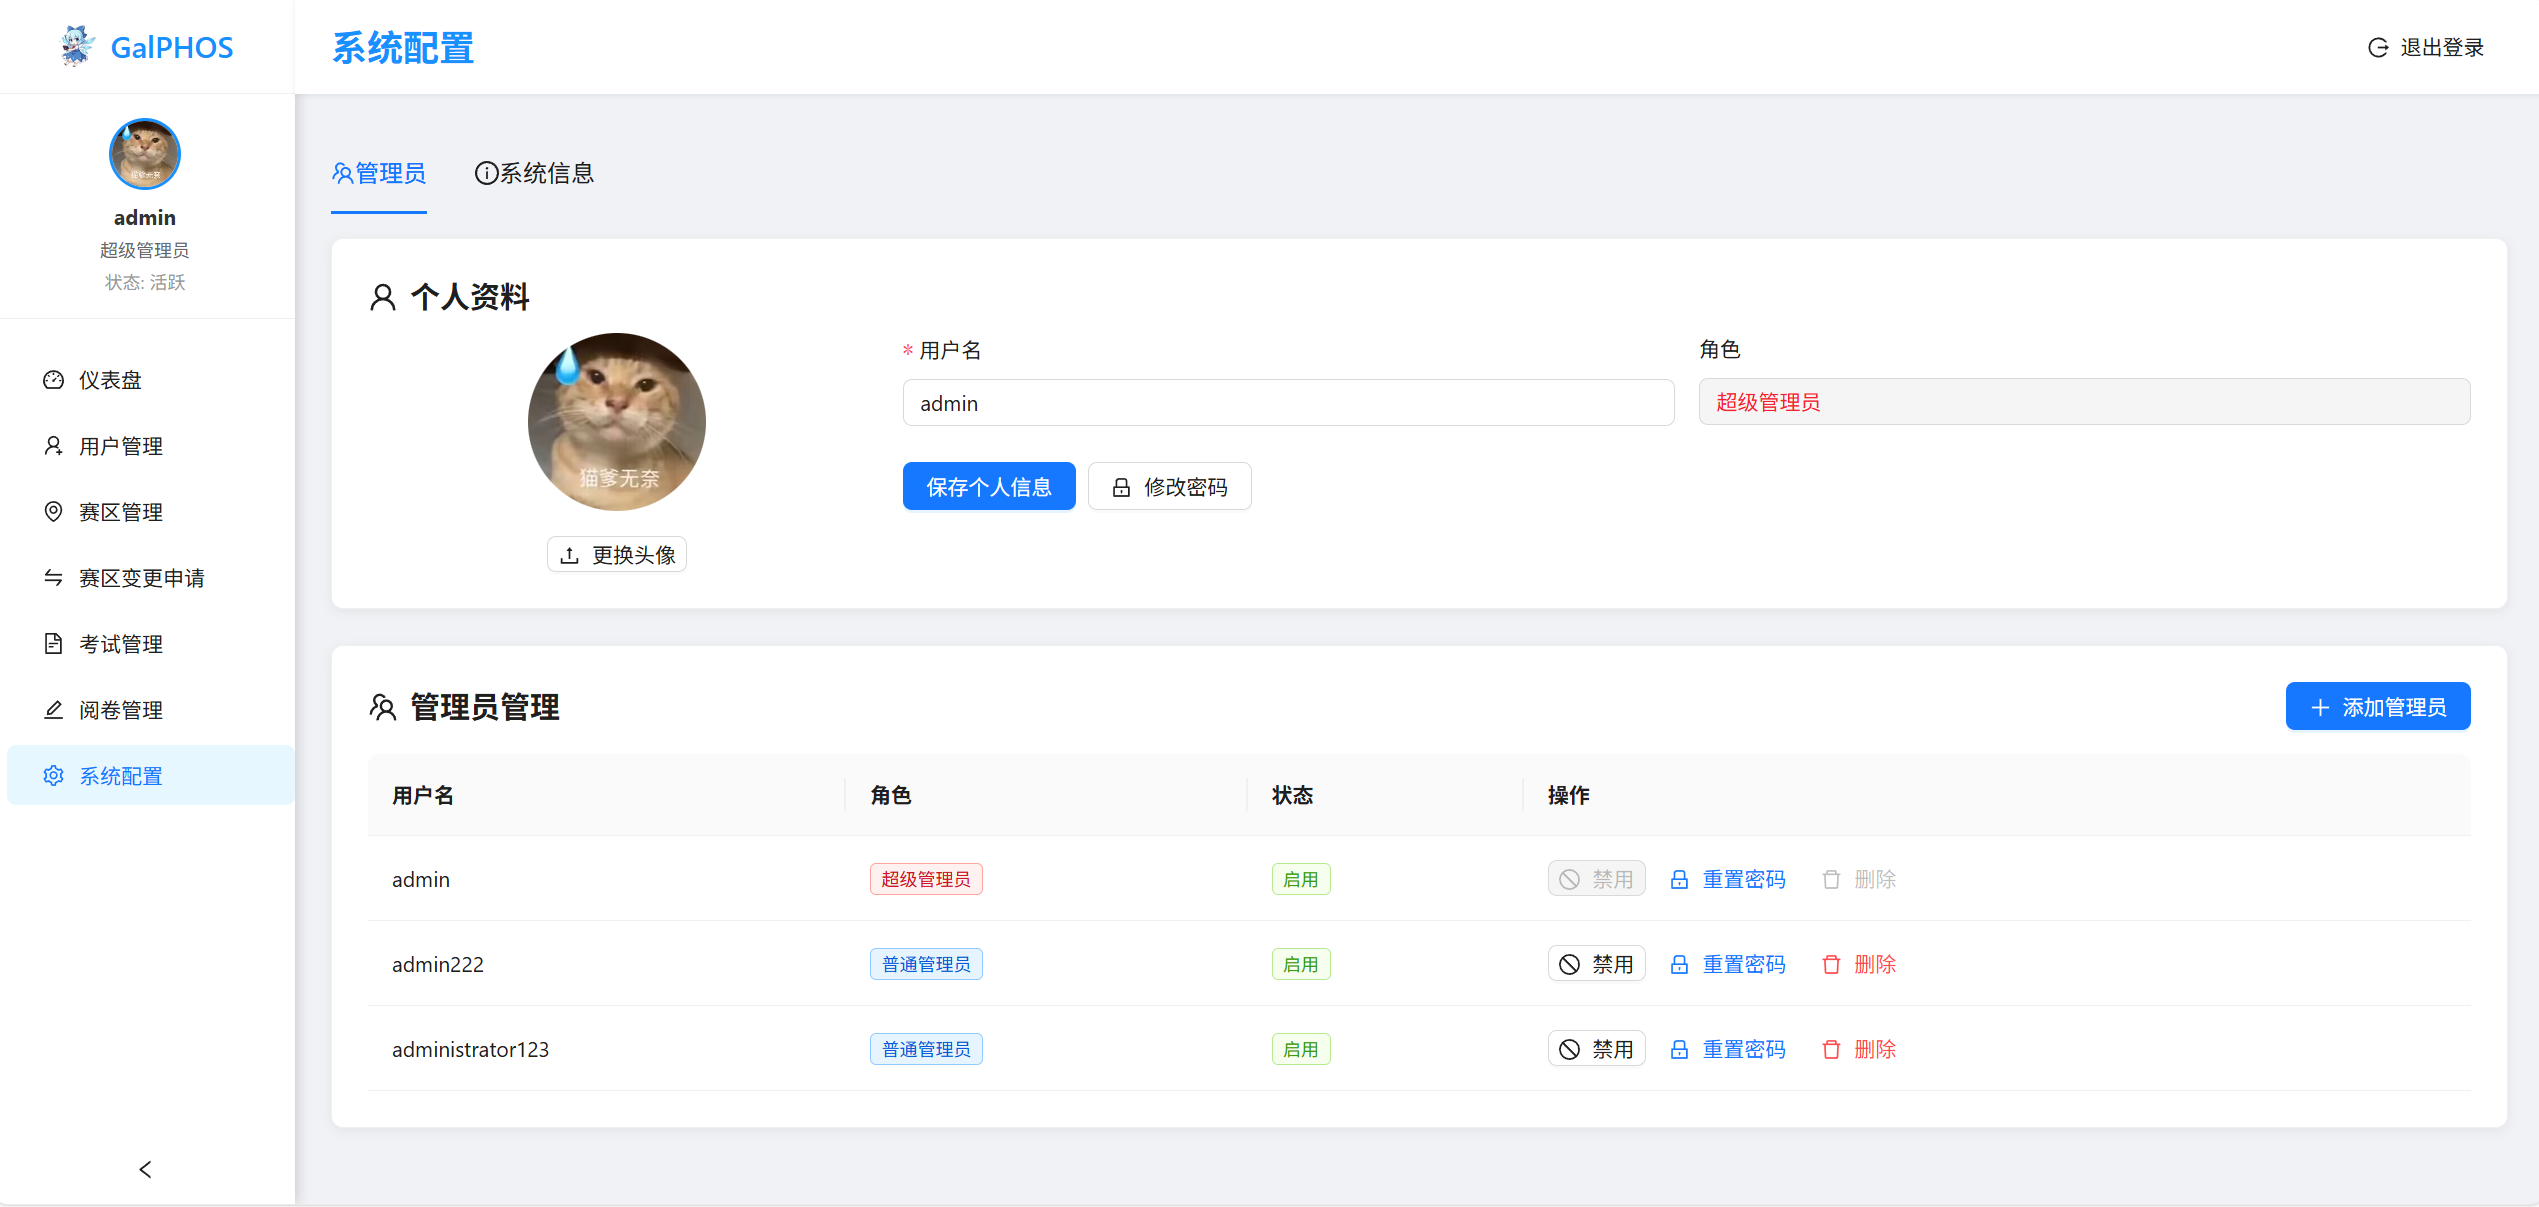
\includegraphics[width=0.75\textwidth]{admin/adminmanage.png}
%     \caption{Admin management page}
%     \label{fig:adminmanage page}
% \end{figure}

Except the admin management
function, the other administrators are able to manage the system in the same way as the super administrator.
\subsubsection{Dashboard}
The admins' dashboard shows information about the system, including the number of registers, number of active users, number of provinces and schools,
information about the exams and so on.
% \begin{figure}[H]
%     \centering
%     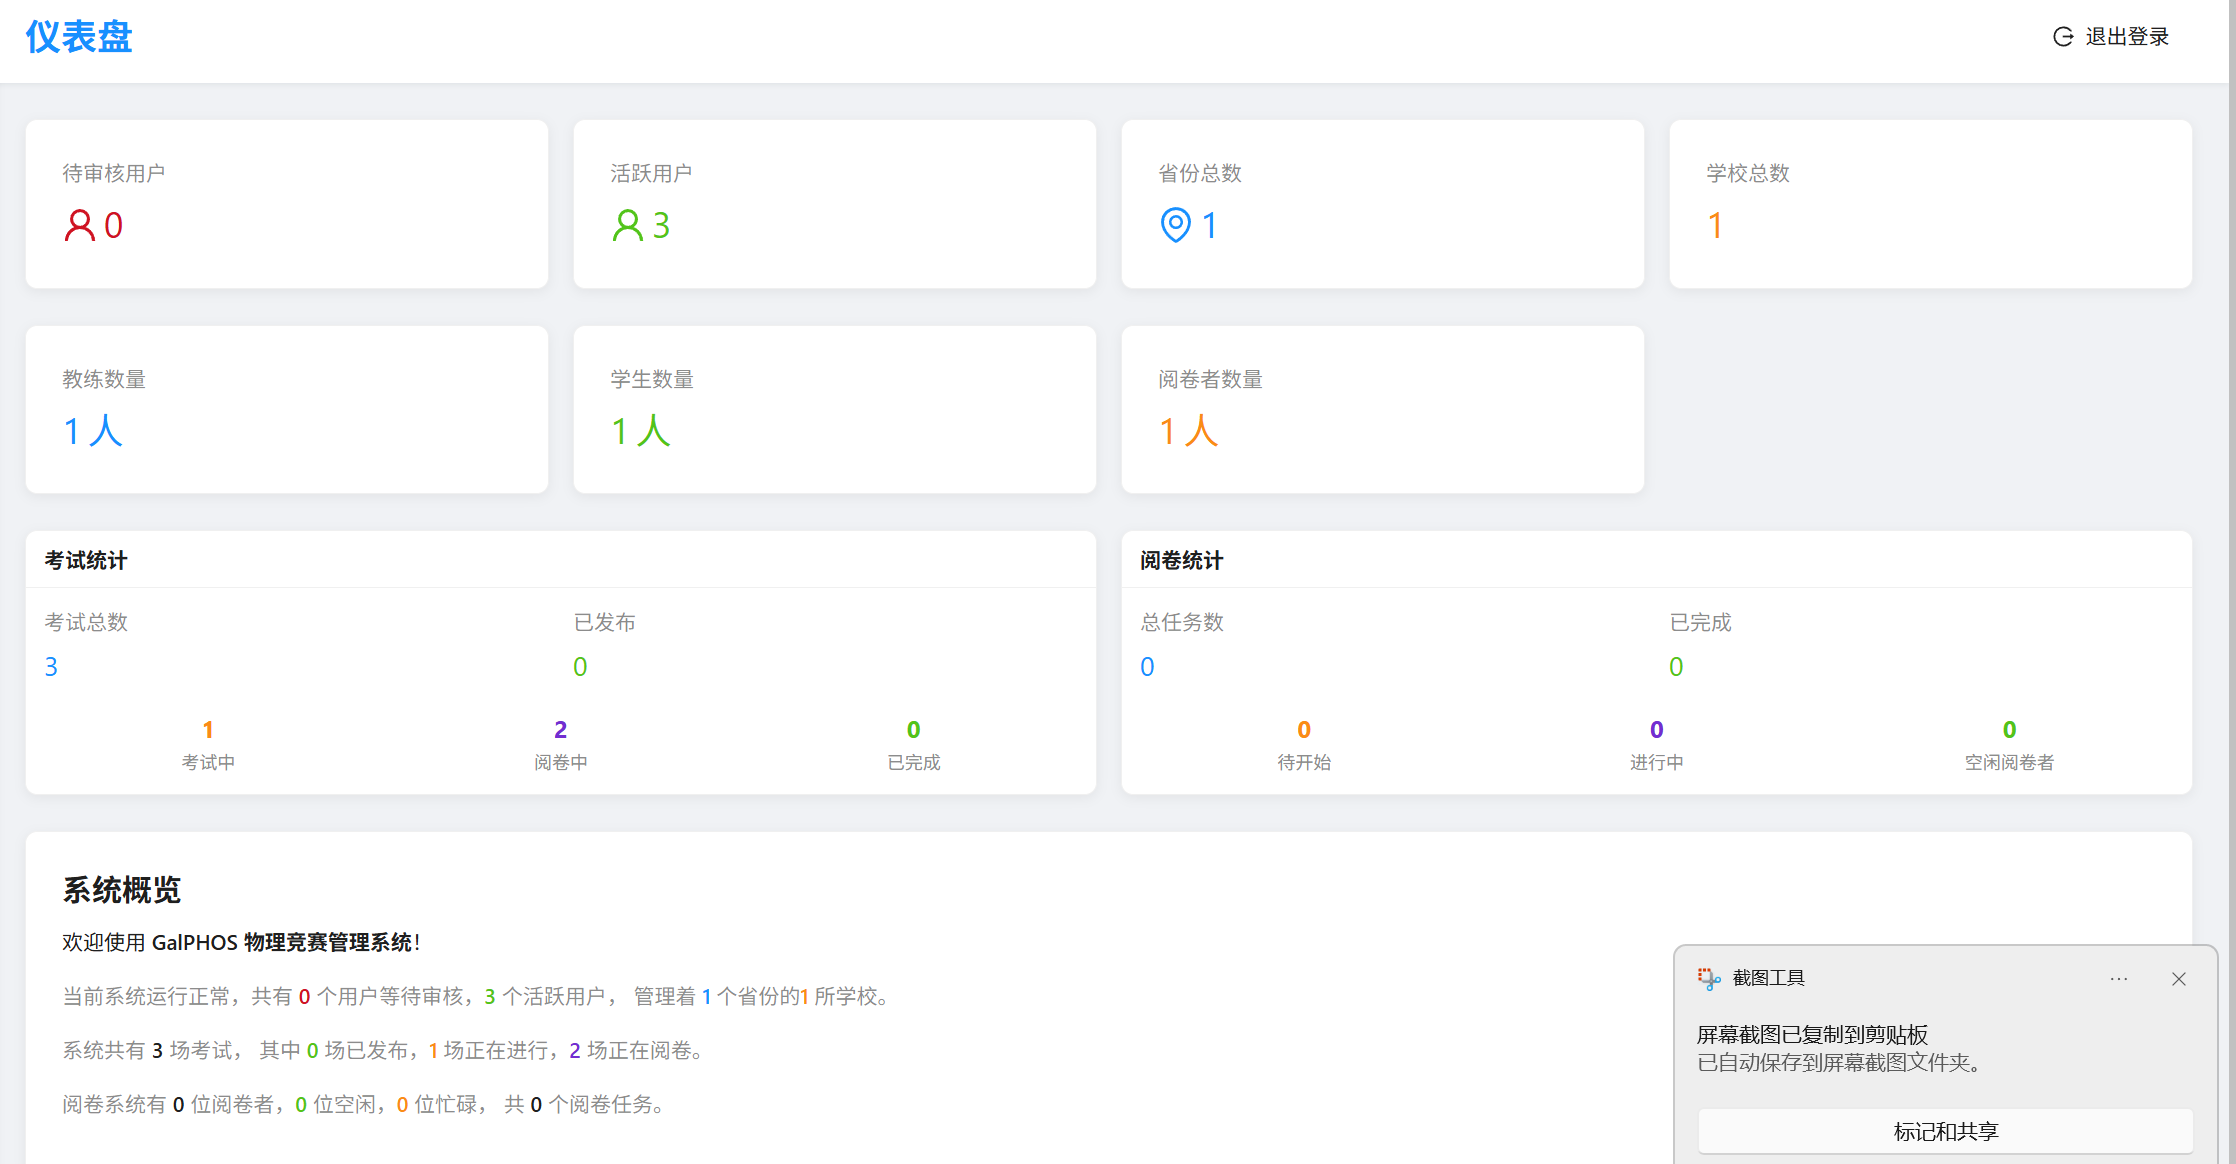
\includegraphics[width=0.75\textwidth]{admin/dashboard4admin.png}
%     \caption{Admin management page}
%     \label{fig:adminmanage page}
% \end{figure}
\subsubsection{User Management}
Administrators can check and manage users in the user management page: administrators can access the detailed information of
the users, including their username, phone number, region, status and other information,
for registering users, administrators can approve or reject their registration requests, and for existing users, administrators can ban or unban them,
and delete them if necessary.
The user management page also provides a search function, allowing administrators to search for users by username, phone number, region,
status and other criteria.
% \begin{figure}[H]
%     \centering
%     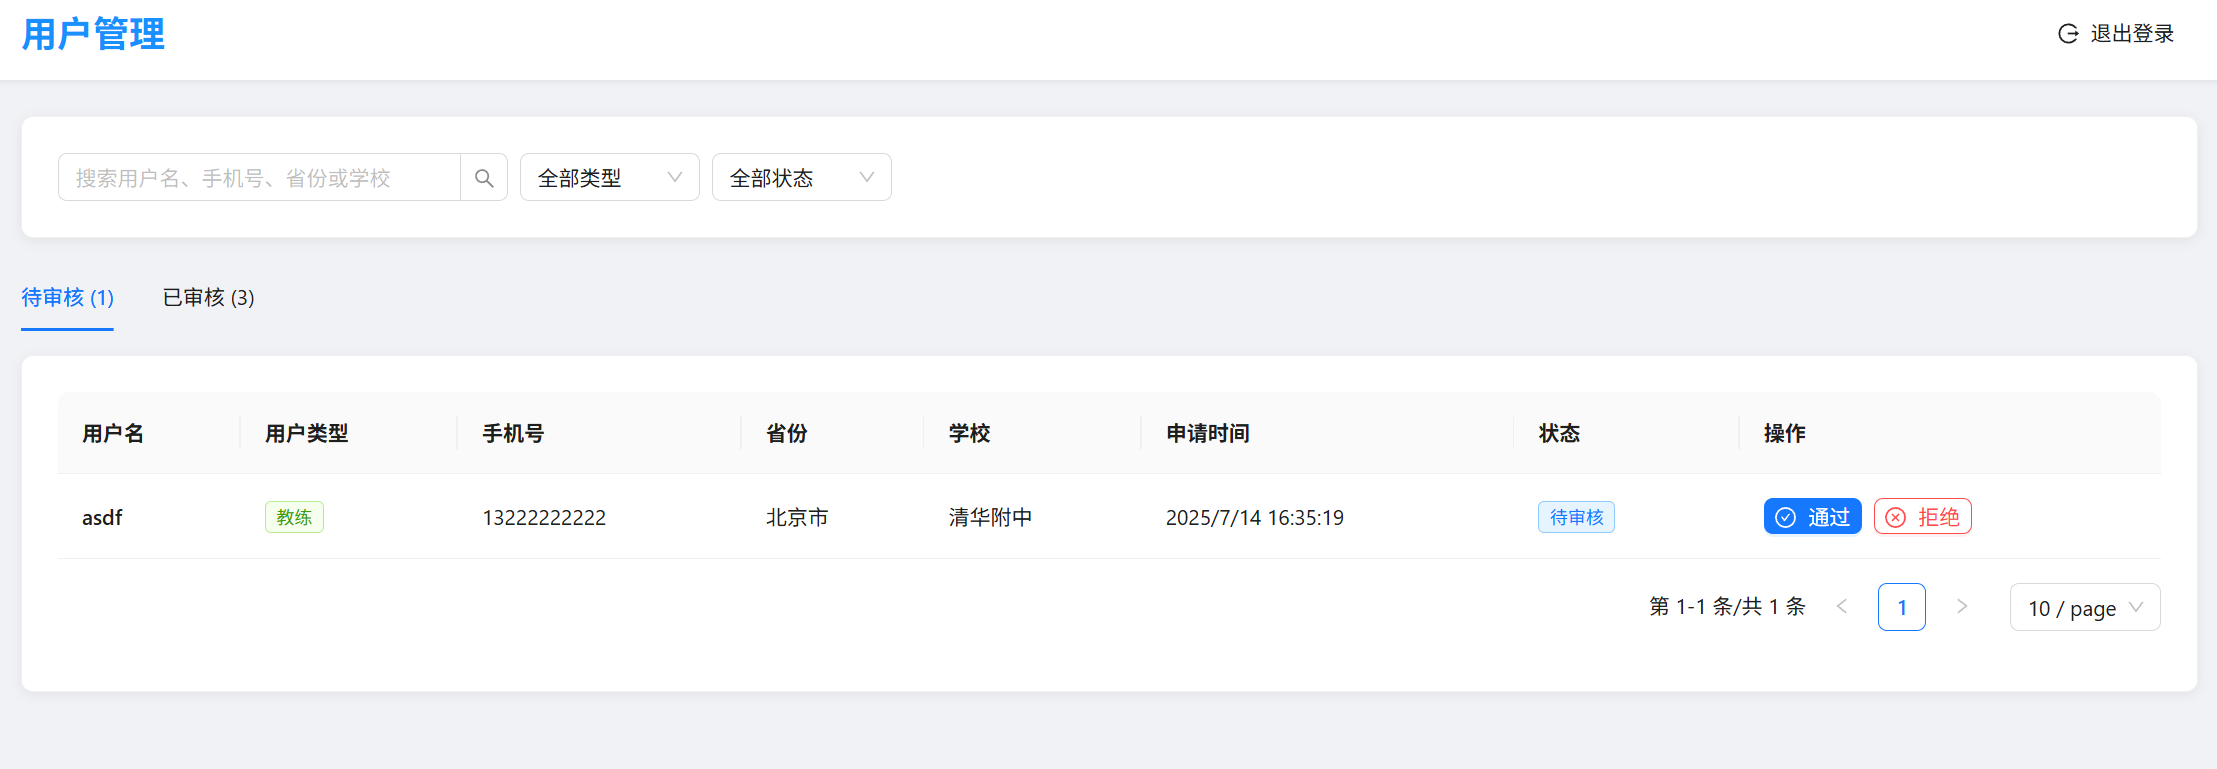
\includegraphics[width=0.8\textwidth]{admin/usermanage-1.png}
%     \caption{UserManagement page: registering users}
%     \label{fig:UserManagement page}
% \end{figure}
% \begin{figure}[H]
%     \centering
%     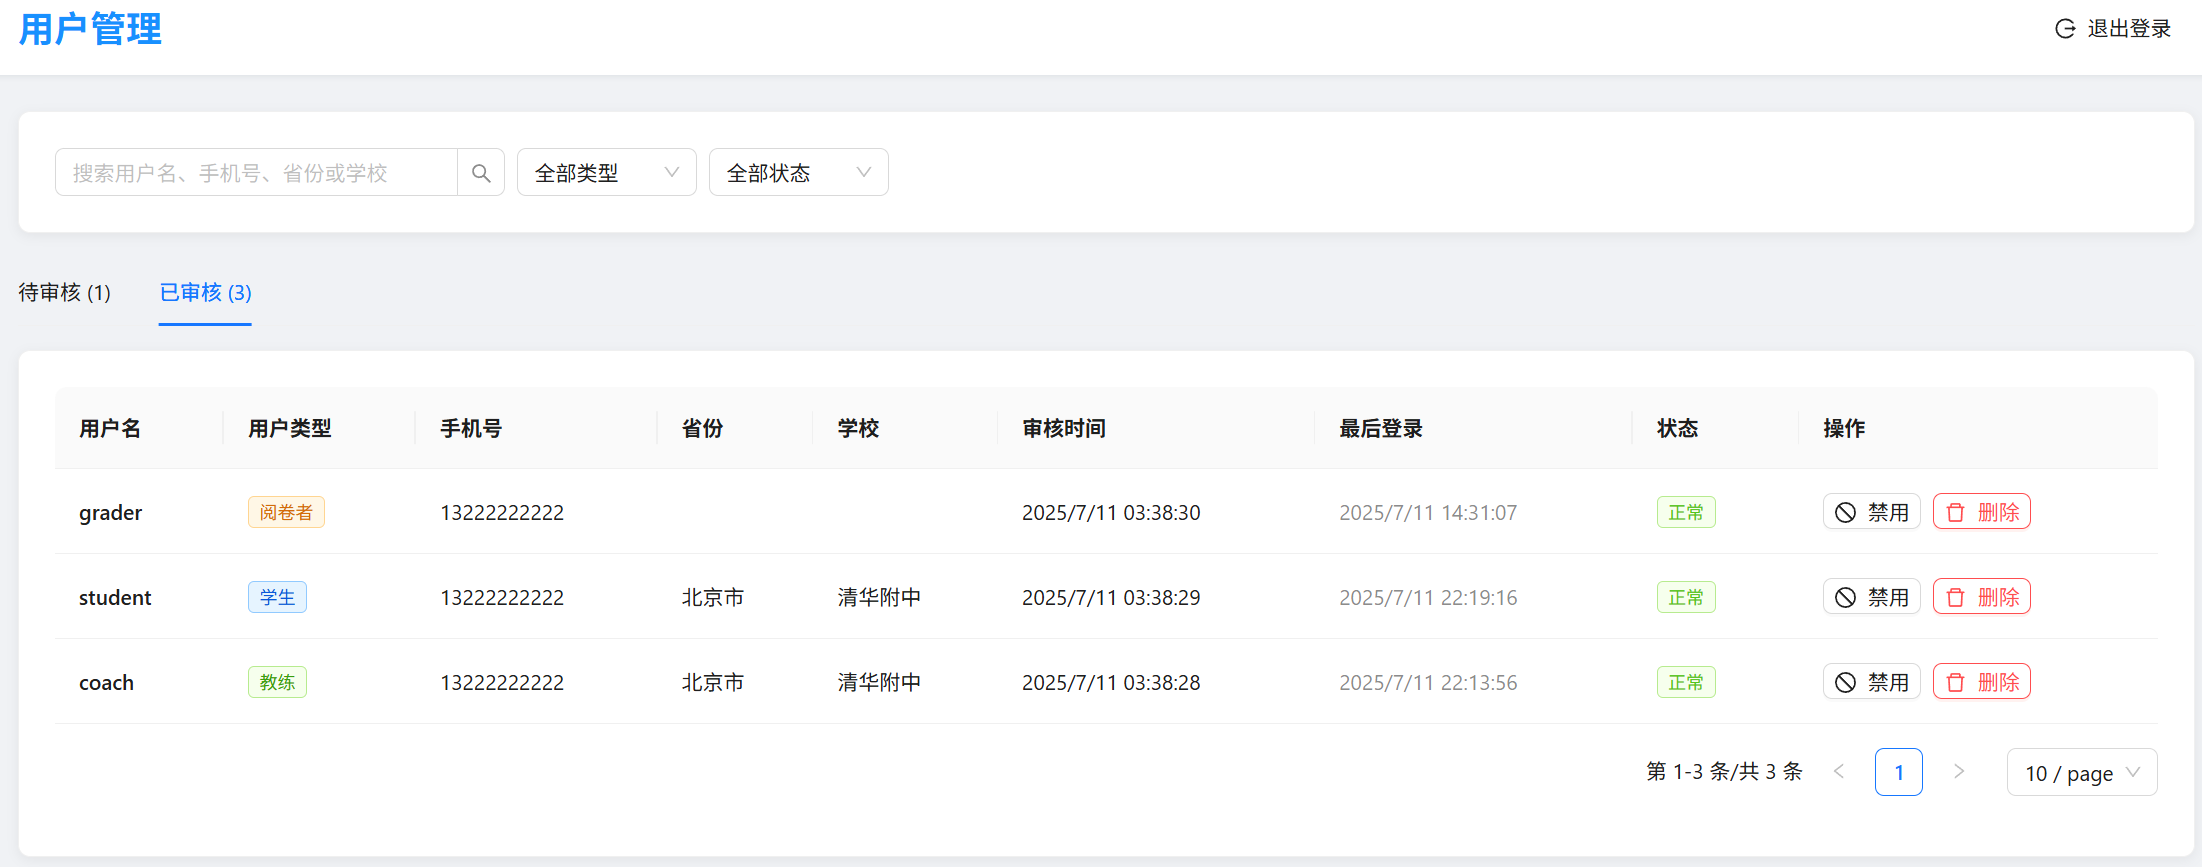
\includegraphics[width=0.8\textwidth]{admin/usermanage-2.png}
%     \caption{UserManagement page: registered users}
%     \label{fig:UserManagement page}
% \end{figure}
\subsubsection{Region Management}
In region management page, administrators can access and manage the active regions and schools in the system. In the 'Province management'
part, administrators can add, delete provinces and add schools to provinces. And in the 'School management' part, administrators can
access the detailed information of the schools, including their name and belonging region.
% \begin{figure}[H]
%     \centering
%     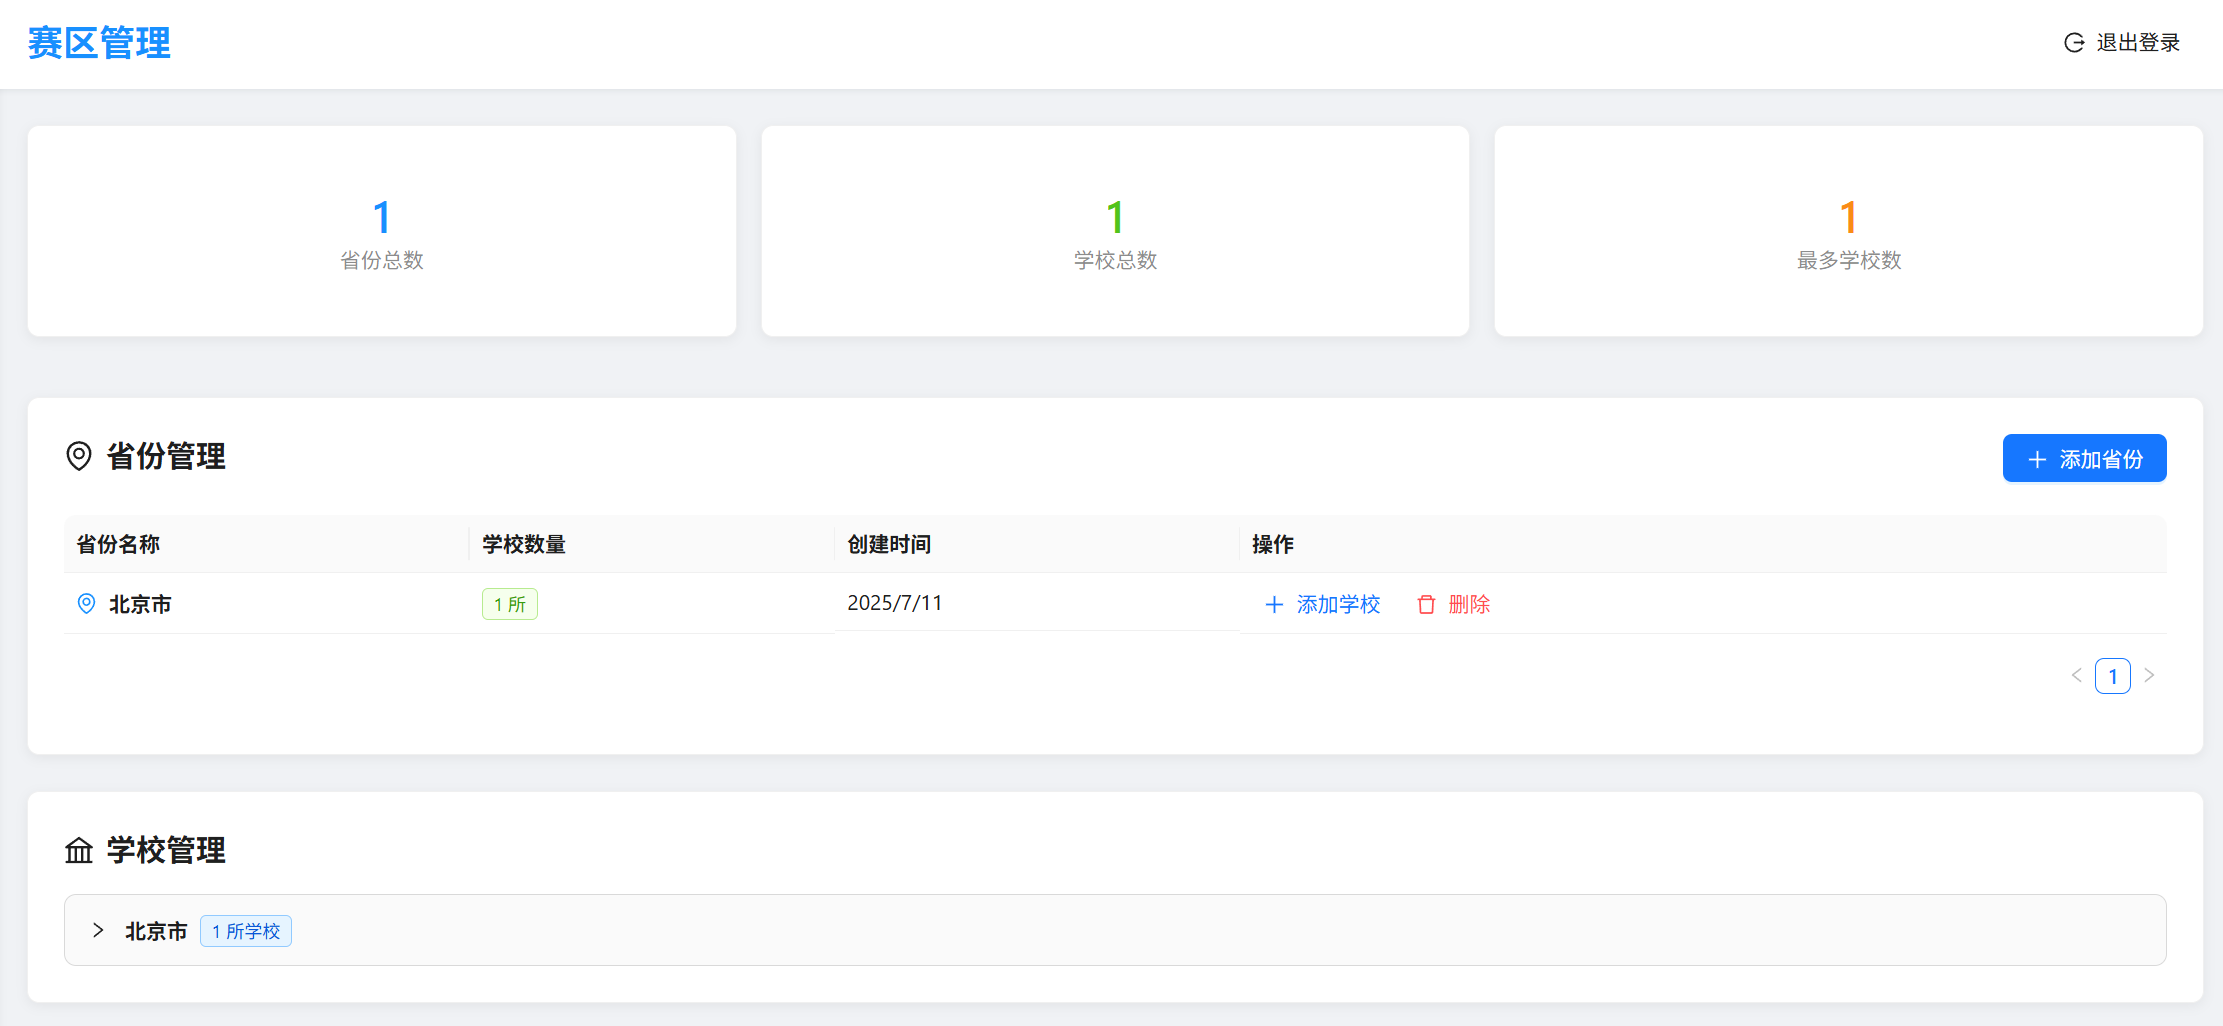
\includegraphics[width=0.75\textwidth]{admin/region-overview.png}
%     \caption{Region management page}
%     \label{fig:RegionManagement page}
% \end{figure}
\subsubsection{Region Changing Management}
In realistic life, some students may change their region or school after registration, so the region changing management page is designed to
manage the region changing requests from students. After the student submits a region changing request,
the administrators can check the request and approve or reject it. If approved, the student's region will be updated accordingly.
This page provides a dashboard showing the number of requests, and a table showing the detailed information of the requests
and allowing administrators to work on the requests on it.
% insert the figure here
% \begin{figure}[H]
%     \centering
%     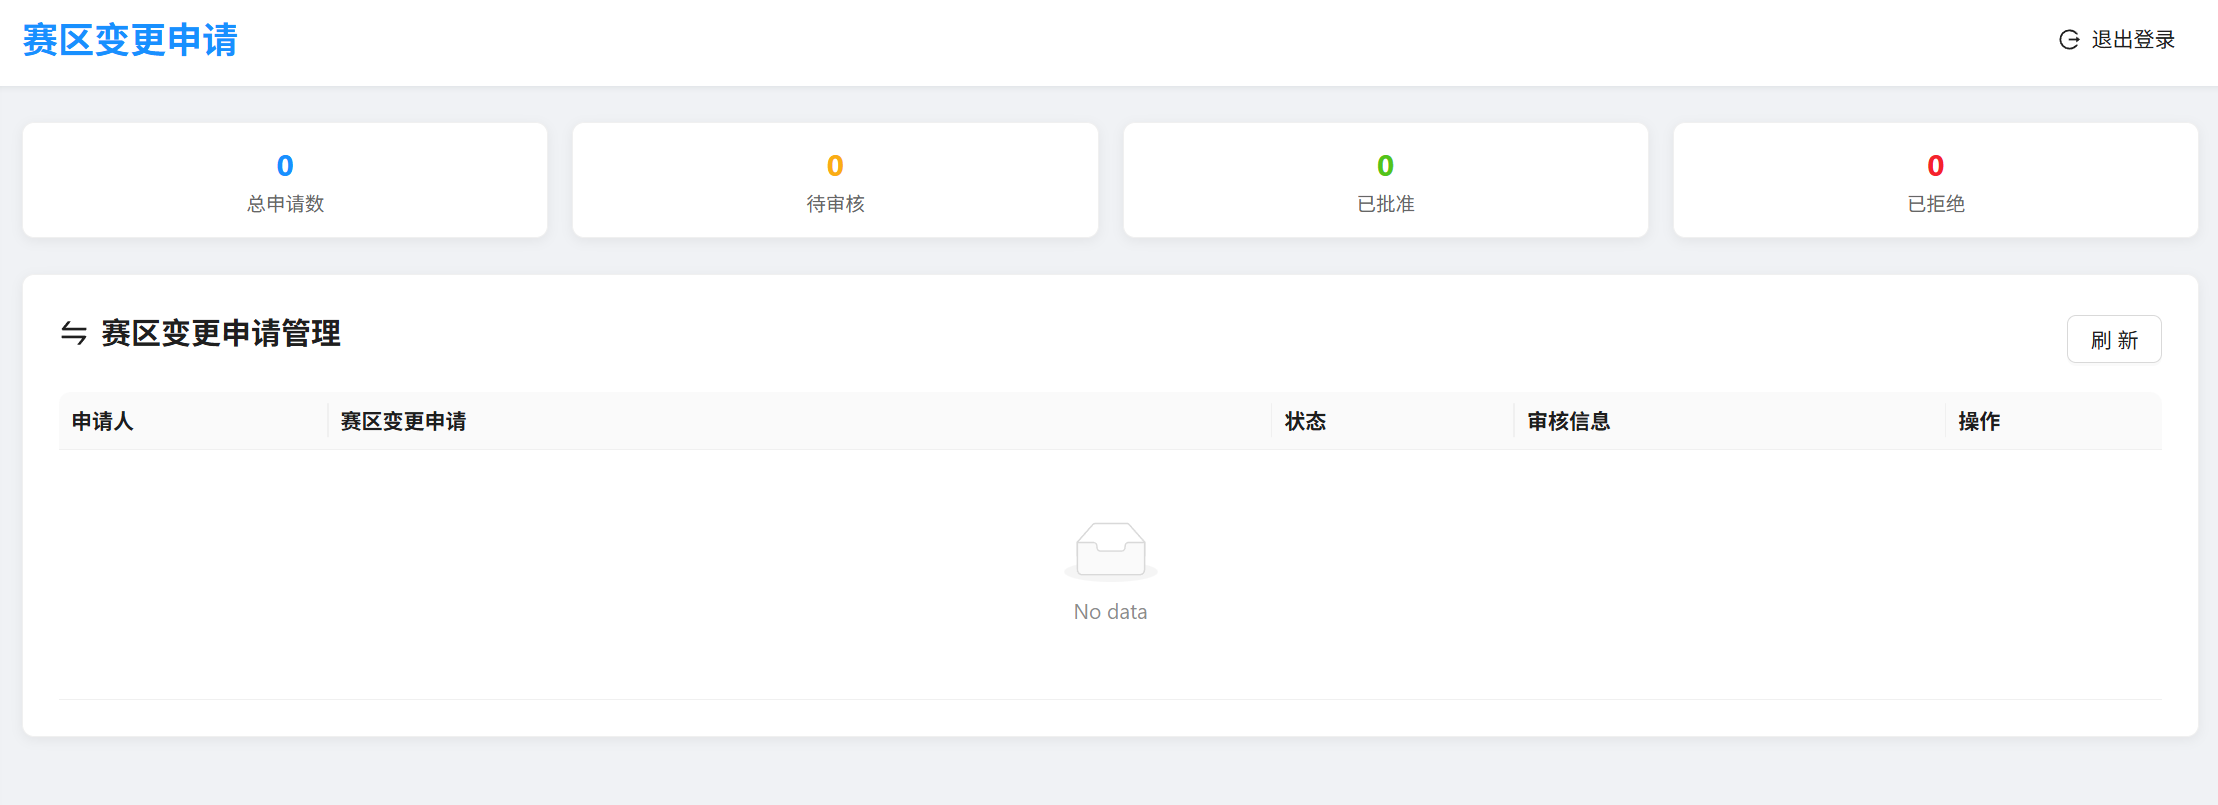
\includegraphics[width=0.8\textwidth]{admin/changeregion.png}
%     \caption{Region changing management page}
%     \label{fig:RegionChangingManagement page}
% \end{figure}
\subsubsection{Exam Management}
The exams are managed by the administrators in the exam management page. Administrators can access the information of the exams, or create, delete and modify exams here.
The dashboard shows the number of exams, and the table shows the detailed information of the exams, including their name, start time, end time, status and other information and
provides a filter function to filter the exams by status.
% \begin{figure}[H]
%     \centering
%     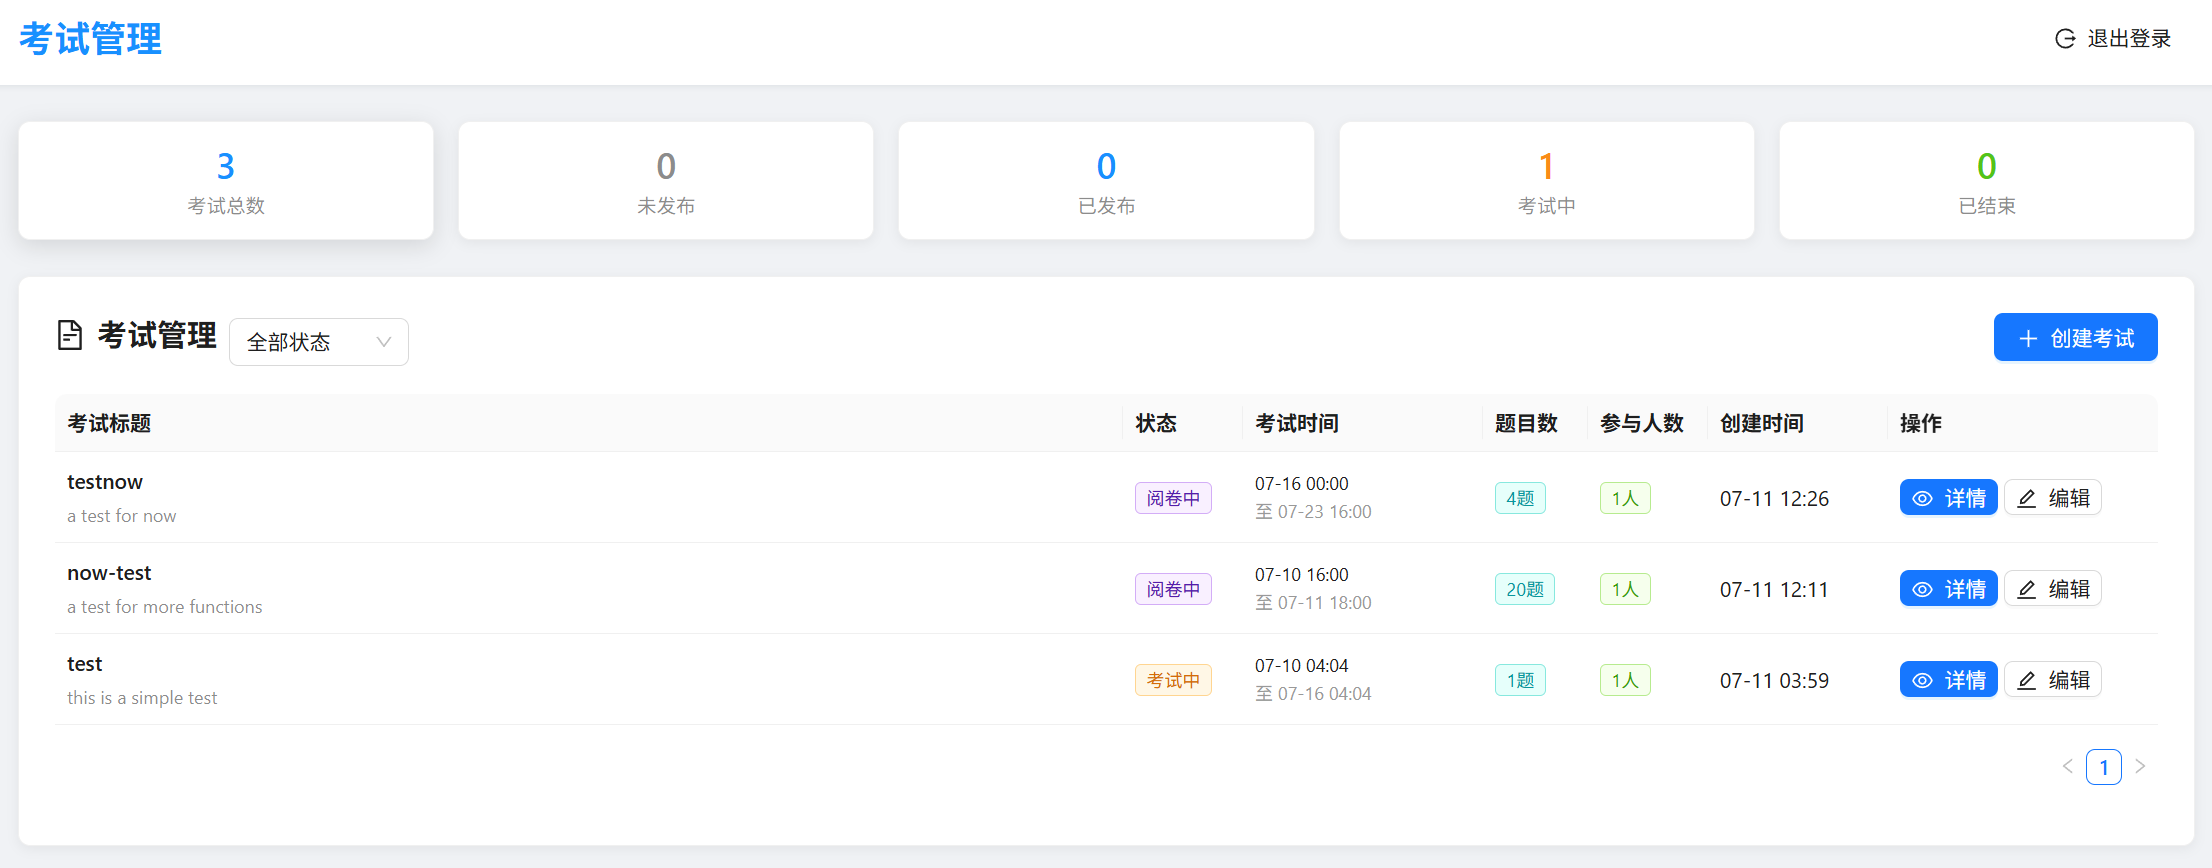
\includegraphics[width=0.8\textwidth]{admin/exammanage.png}
%     \caption{Exam management page overview}
%     \label{fig:ExamManagement page}
% \end{figure}
The exams have total five states: 'Not Published', 'Published', 'In Progress', 'Finished' and 'Graded'.
To create an exam, administrators need to provide basic exam information: title, detailed information, number of questions, total score,
time limit, start time and end time, and the files of test paper, answer sheet and solution.
% \begin{figure}[H]
%     \centering
%     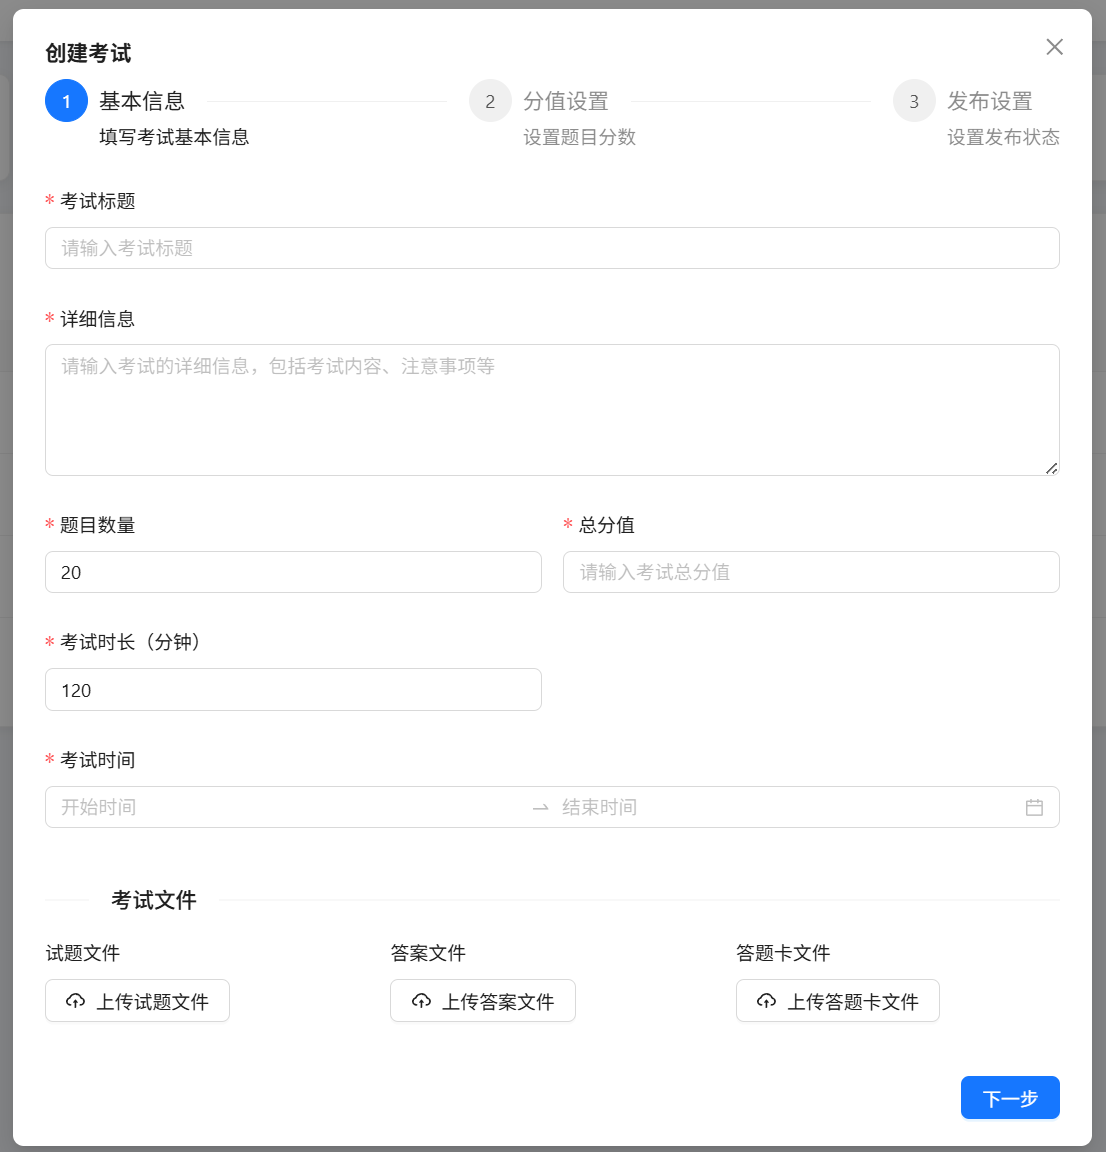
\includegraphics[width=\textwidth]{admin/createexam1.png}
%     \caption{Exam creation page and file upload}
%     \label{fig:ExamCreation page}
% \end{figure}
% \begin{figure}[H]
%     \centering
%     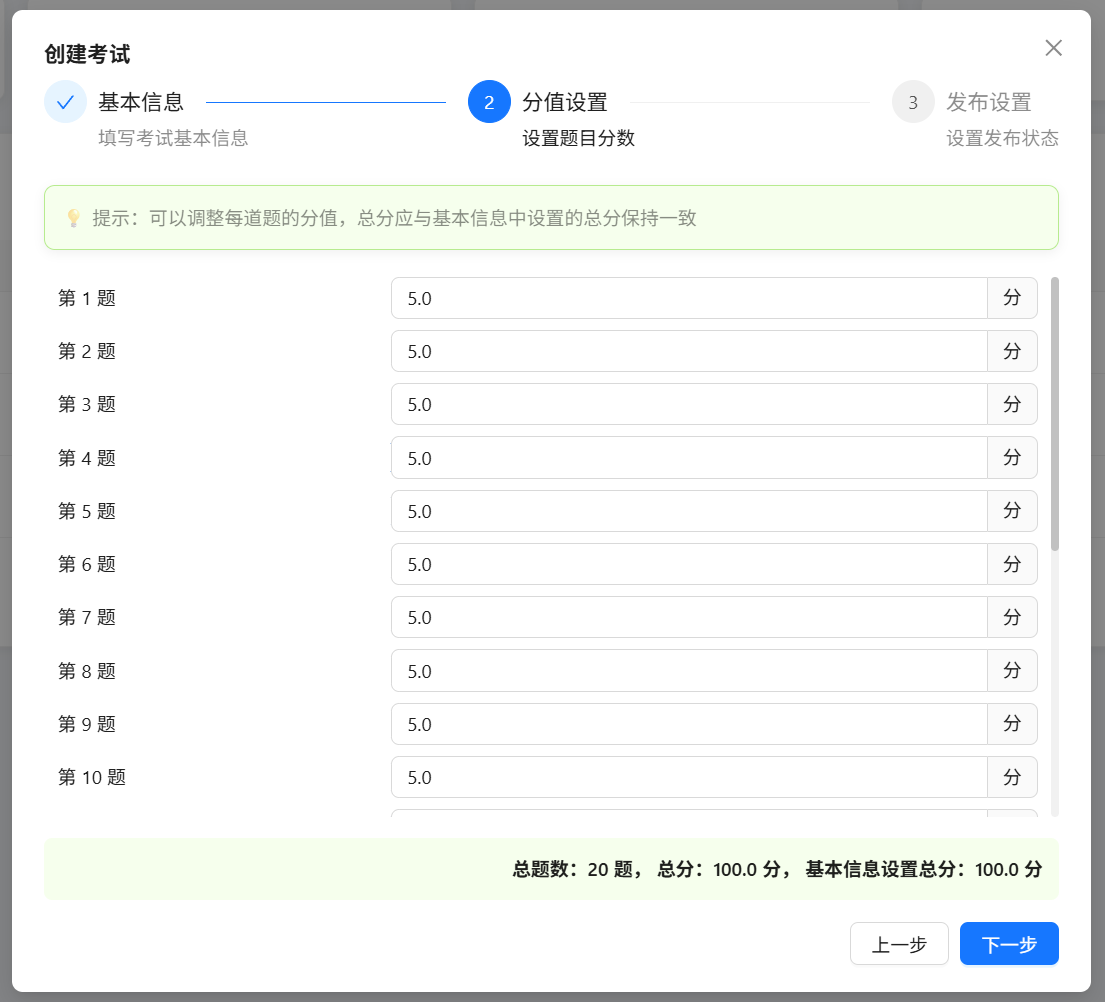
\includegraphics[width=\textwidth]{admin/createexam2.png}
%     \caption{Exam creation page: grade setting}
%     \label{fig:ExamCreation page2}
% \end{figure}
% \begin{figure}[H]
%     \centering
%     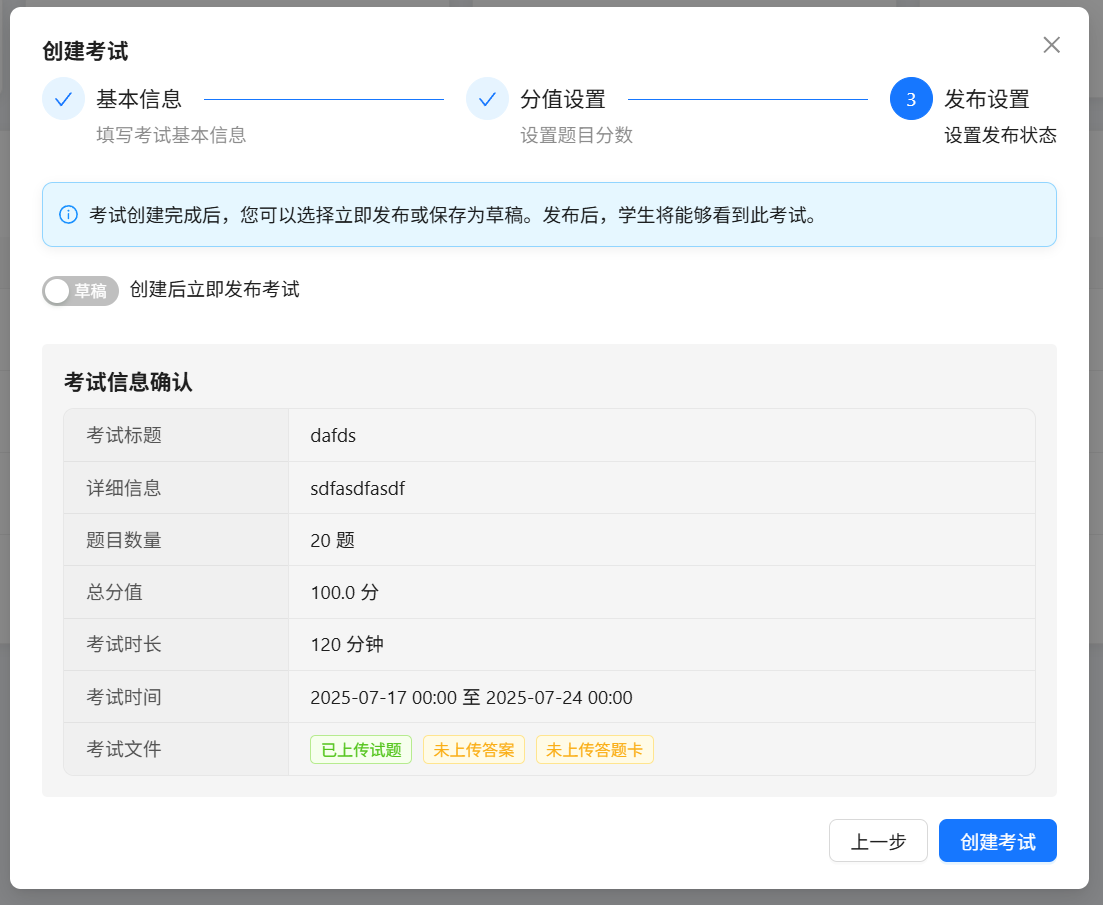
\includegraphics[width=\textwidth]{admin/createexam3.png}
%     \caption{Exam creation page: final confirmation}
%     \label{fig:ExamCreation page3}
% \end{figure}
% After setting up the exam, administrators can preview the exam and check the information before creating it.
% \begin{figure}[H]
%     \centering
%     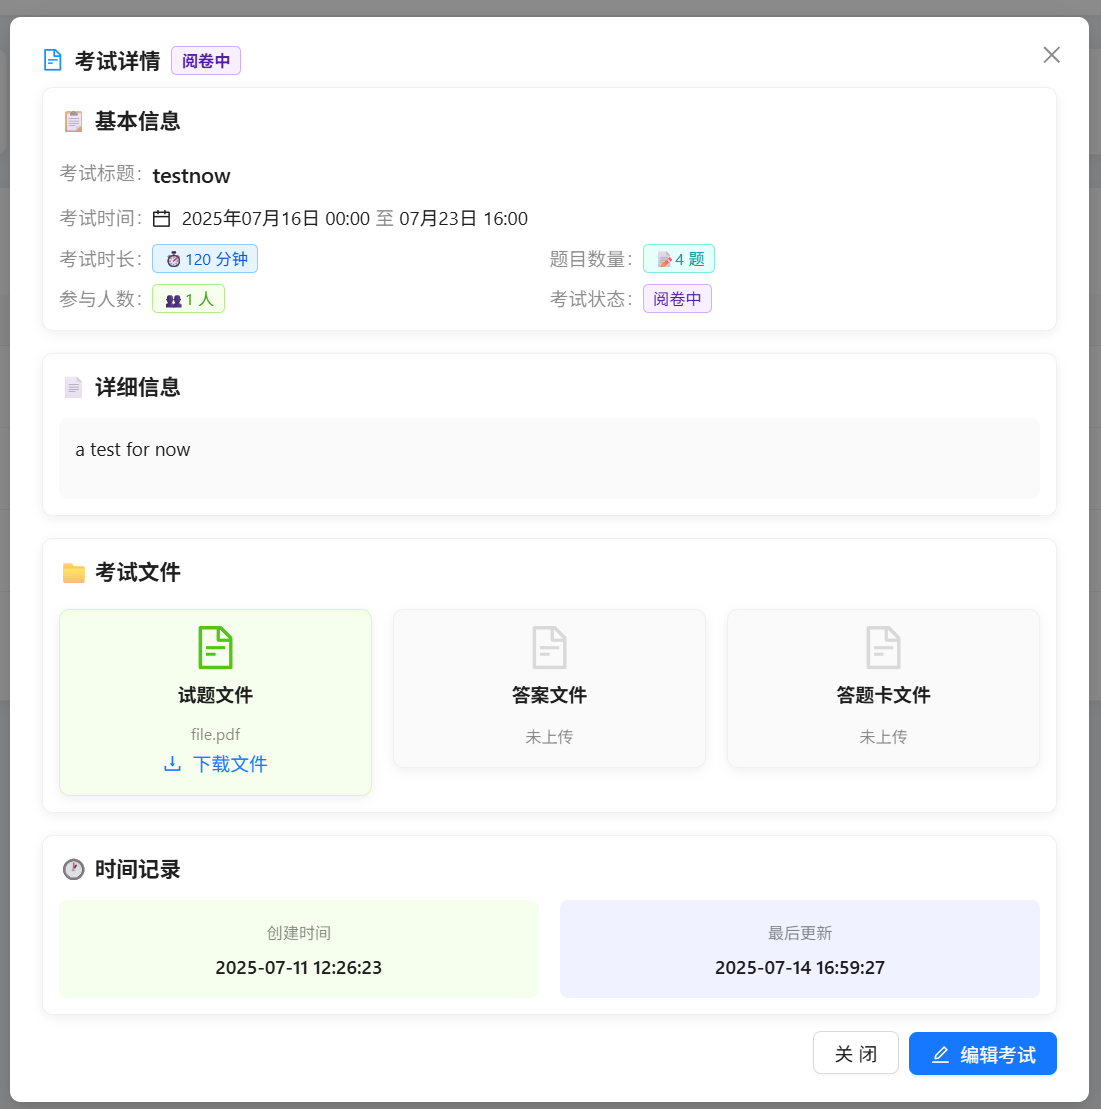
\includegraphics[width=\textwidth]{admin/checkexam.png}
%     \caption{Exam creation page: exam created}
%     \label{fig:ExamCreation page4}
% \end{figure}


% \begin{figure}[htbp]
%   \centering
%   \setlength{\tabcolsep}{0pt}  % 去除表格列间距
%   \renewcommand{\arraystretch}{0}  % 去除表格行间距
  
%   \begin{tabular}{cc}
%     % 左上
%     \begin{subfigure}[t]{0.45\textwidth}
%       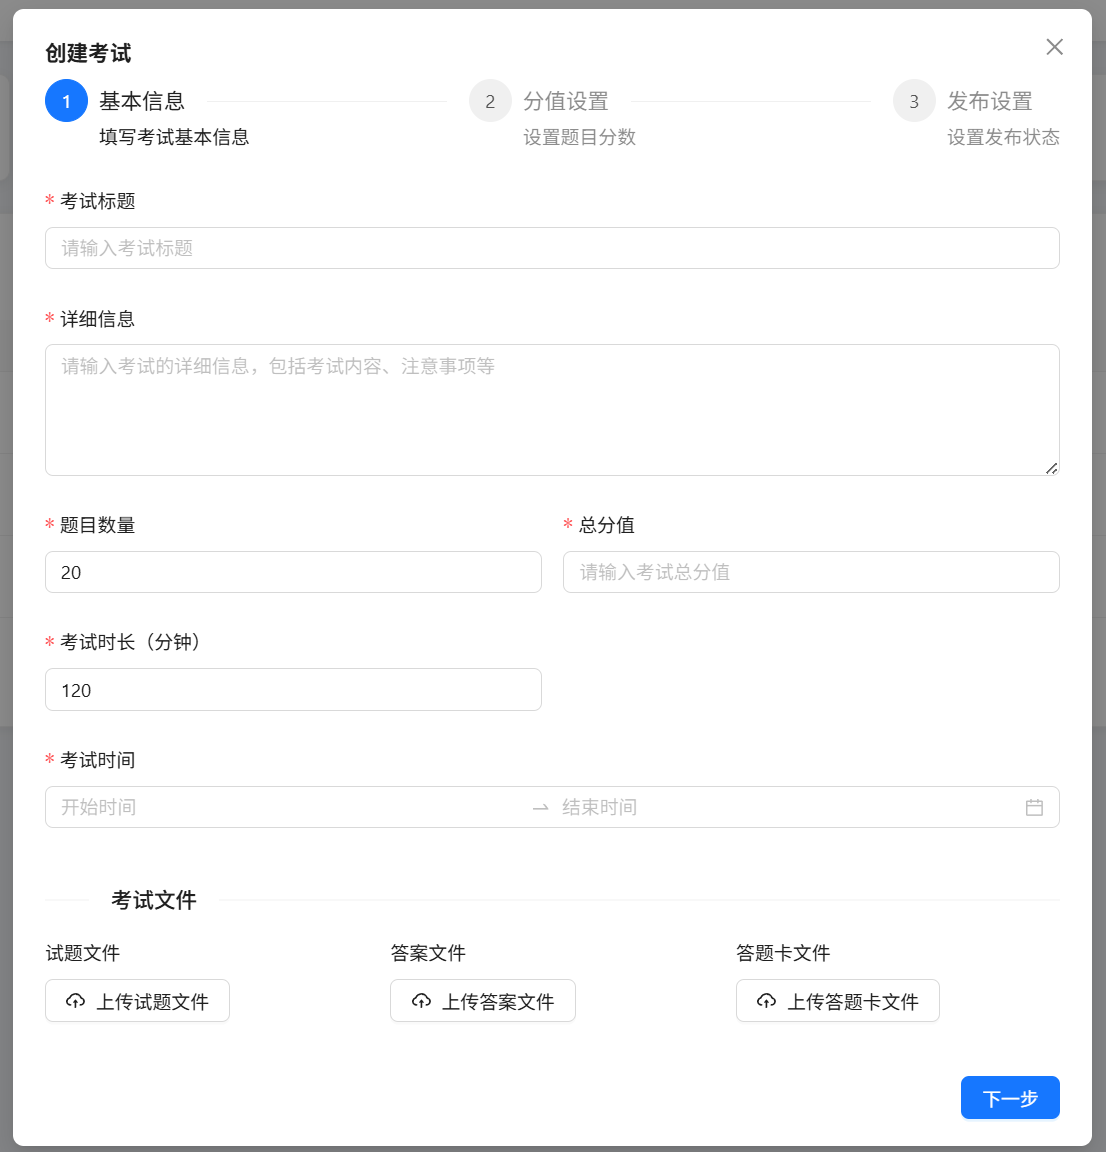
\includegraphics[width=\textwidth,height=4cm,keepaspectratio]{admin/createexam1.png}
%       \caption*{图1}
%     \end{subfigure} &
%     % 右上
%     \begin{subfigure}[t]{0.45\textwidth}
%       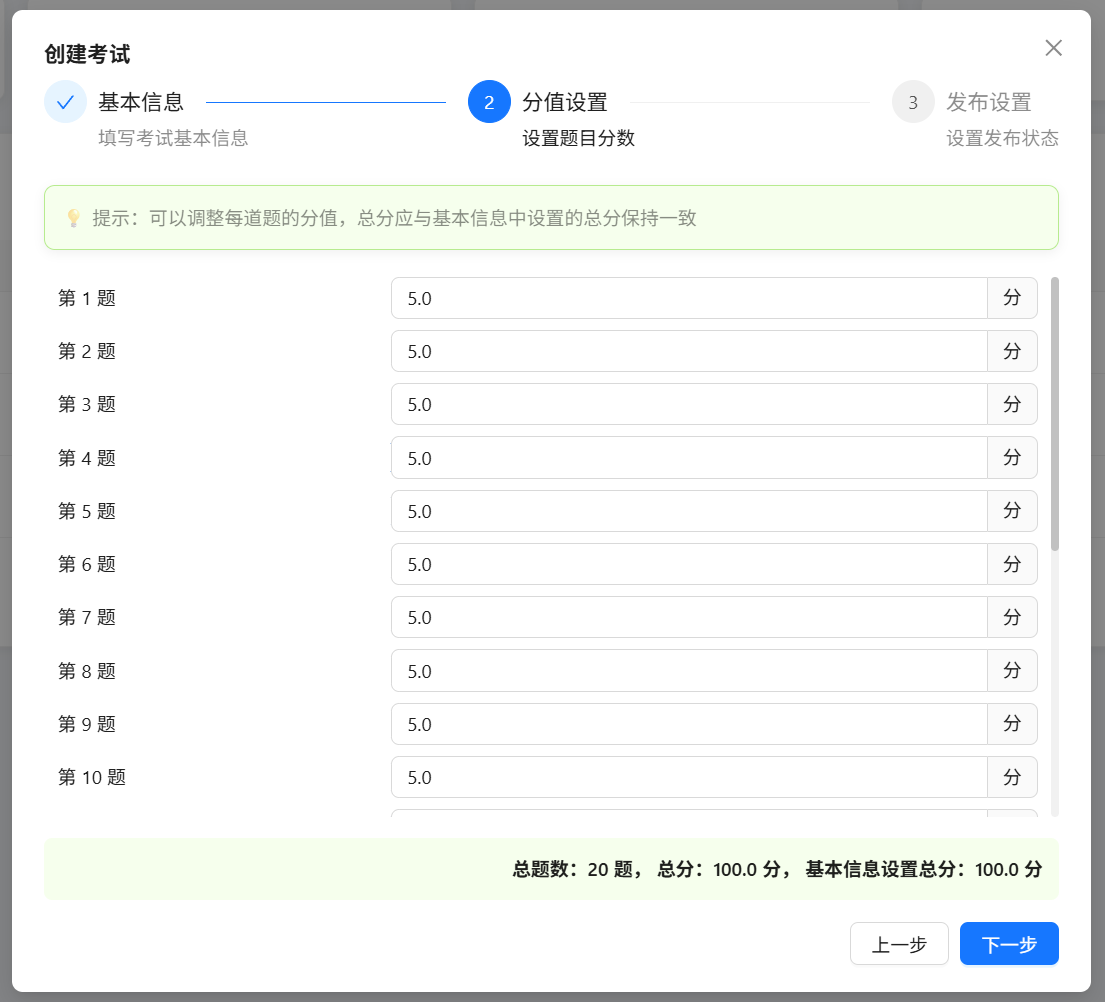
\includegraphics[width=\textwidth,height=4cm,keepaspectratio]{admin/createexam2.png}
%       \caption*{图2}
%     \end{subfigure} \\
%     % 左下
%     \begin{subfigure}[t]{0.45\textwidth}
%       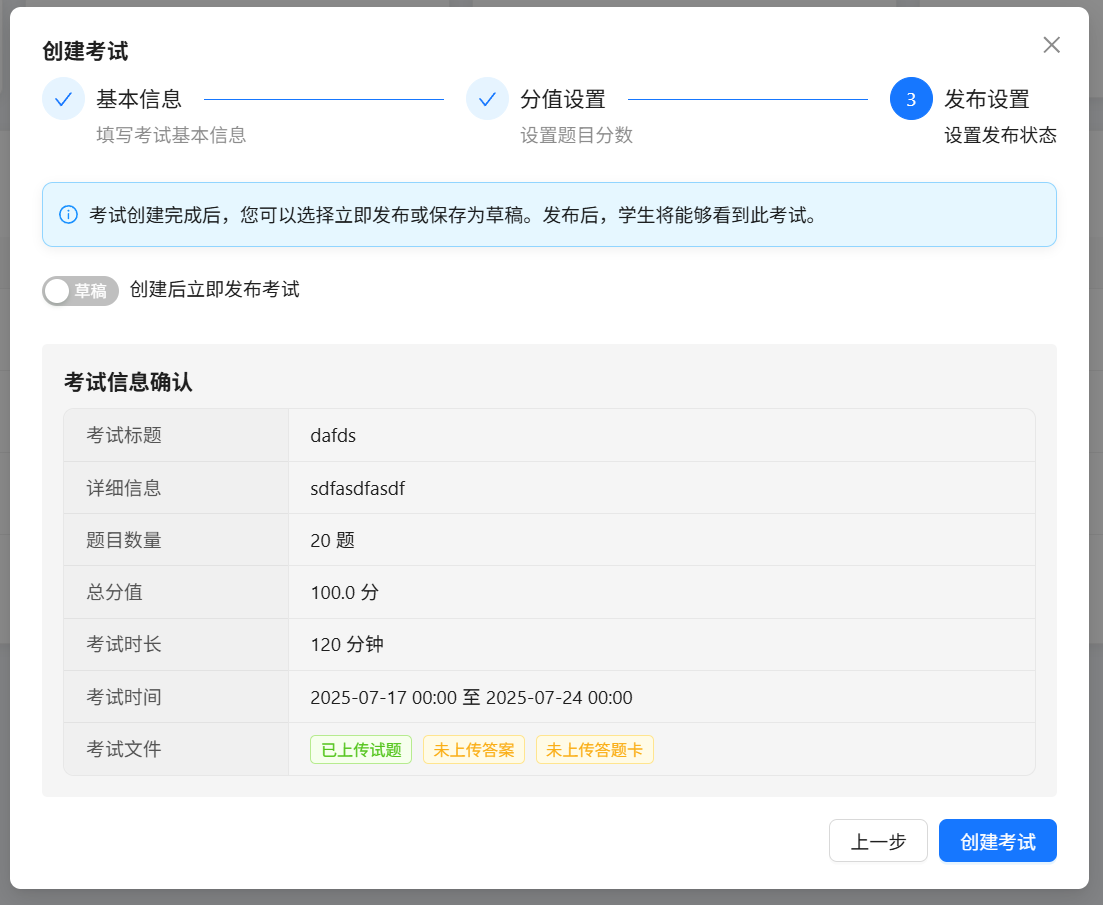
\includegraphics[width=\textwidth,height=4cm,keepaspectratio]{admin/createexam3.png}
%       \caption*{图3}
%     \end{subfigure} &
%     % 右下
%     \begin{subfigure}[t]{0.45\textwidth}
%       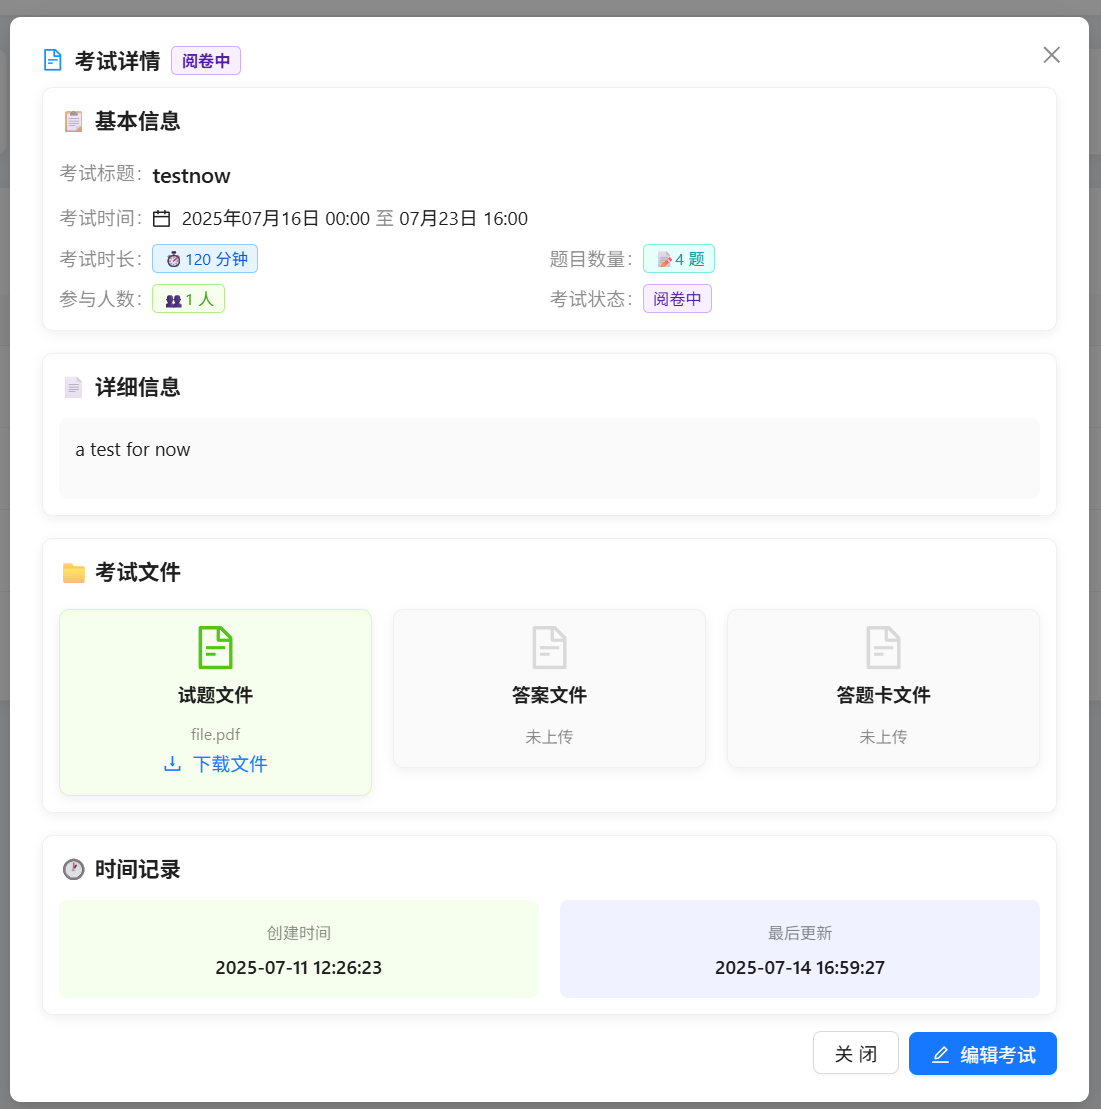
\includegraphics[width=\textwidth,height=4cm,keepaspectratio]{admin/checkexam.png}
%       \caption*{图4}
%     \end{subfigure}
%   \end{tabular}
  
%   \caption{四张图片的紧凑组合}
%   \label{fig:compact-four}
% \end{figure}



We also provide the function to save
current exam as a draft with the state 'Not Published', so that administrators can modify it later.
After the exam is published, other users can see the exam in their pages, and the exam will automatically change its state to 'In Progress' when the start time is reached and
end its state to 'Finished' when the end time is reached. Only when in the 'In Progress' state, students can submit their answer.
In the 'Finished' state, the answer sheets can be distributed to the graders by the administrator and the graders can grade the answer sheets in the 'Graded' state.
After all answer sheets are graded, the exam will automatically change its state to 'Graded', and the results will be calculated and stored in the database
so that users can check their results later.
\subsubsection{Grading Management}
After a exam is finished, the administrators can distribute the answer sheets to the graders in the grading management page.
In this page, administrators can check the current status of the system, including the number of answer sheets to be graded, the number of graders,
and the progress of grading. The administrators can assign different questions to different graders, while the grading service
will automatically assign the questions to the graders based on their availability and workload.
% \begin{figure}[H]
%     \centering
%     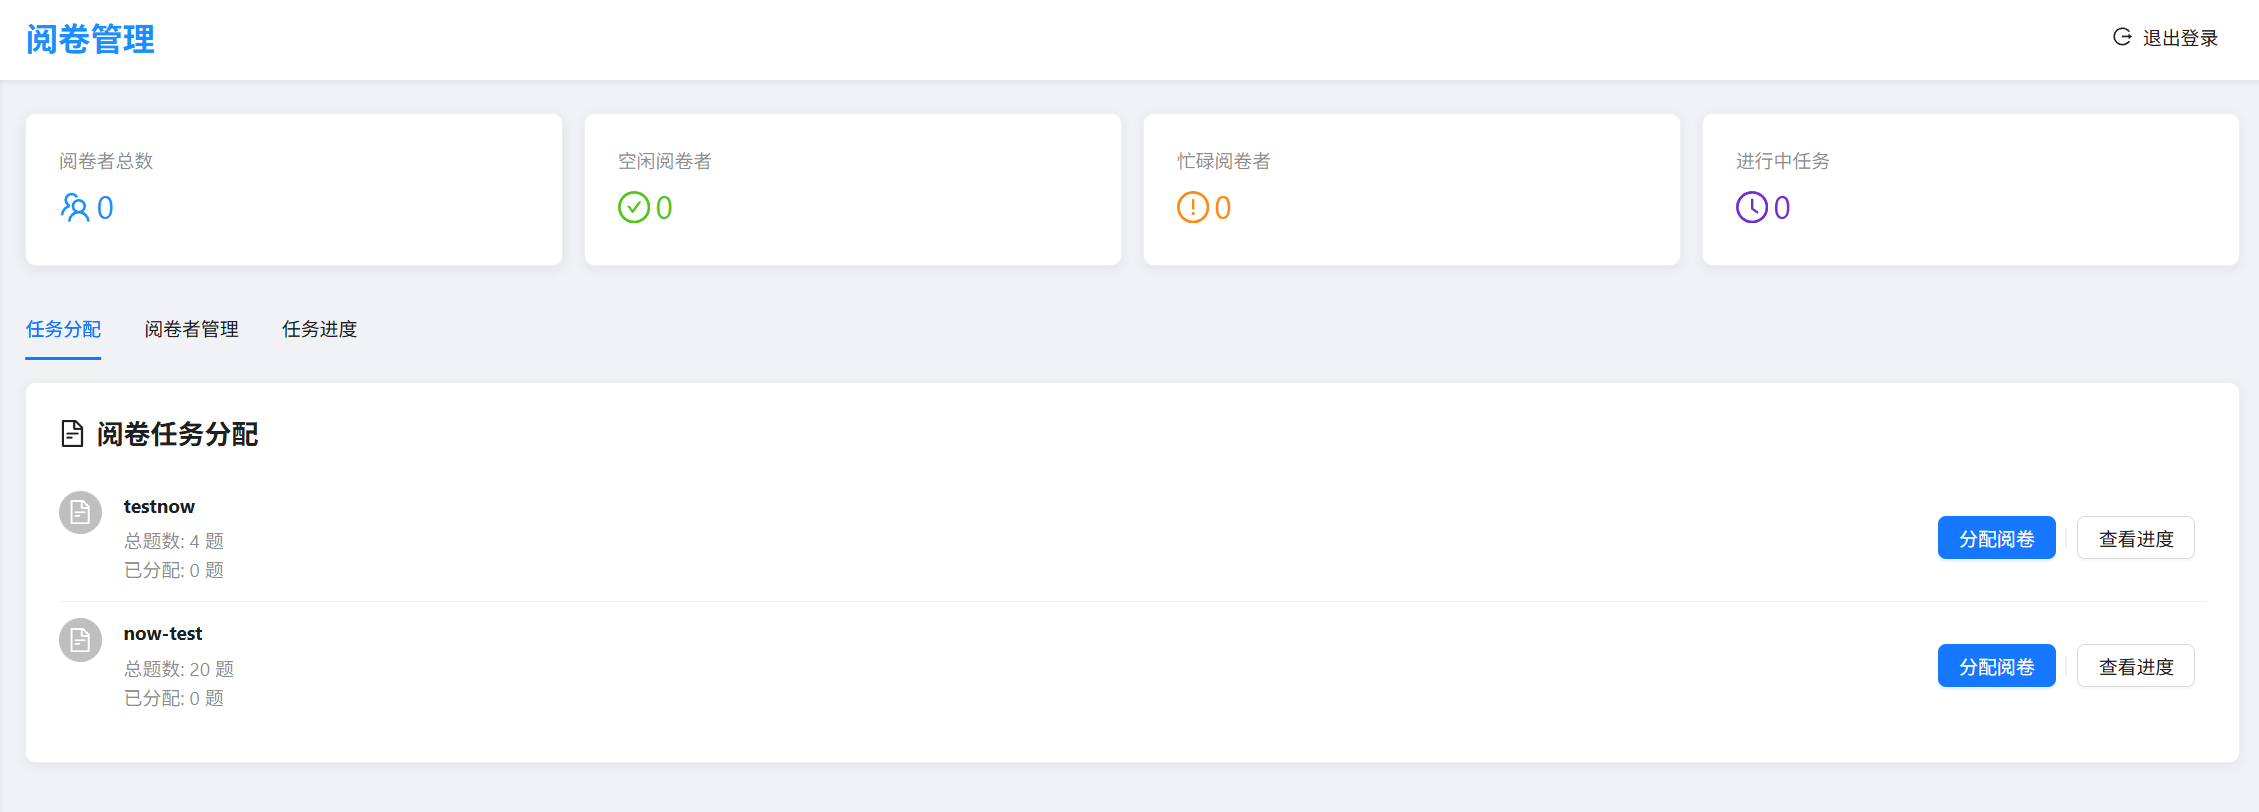
\includegraphics[width=0.8\textwidth]{admin/gradermanage.png}
%     \caption{Grading management page}
%     \label{fig:GradingManagement page}
% \end{figure}
\subsection{Student}
\subsubsection{Dashboard}
The students' dashboard shows the information about the ongoing and finished exams, including the grades of the finished exams and the status of the ongoing exams.
% \begin{figure}[H]
%     \centering
%     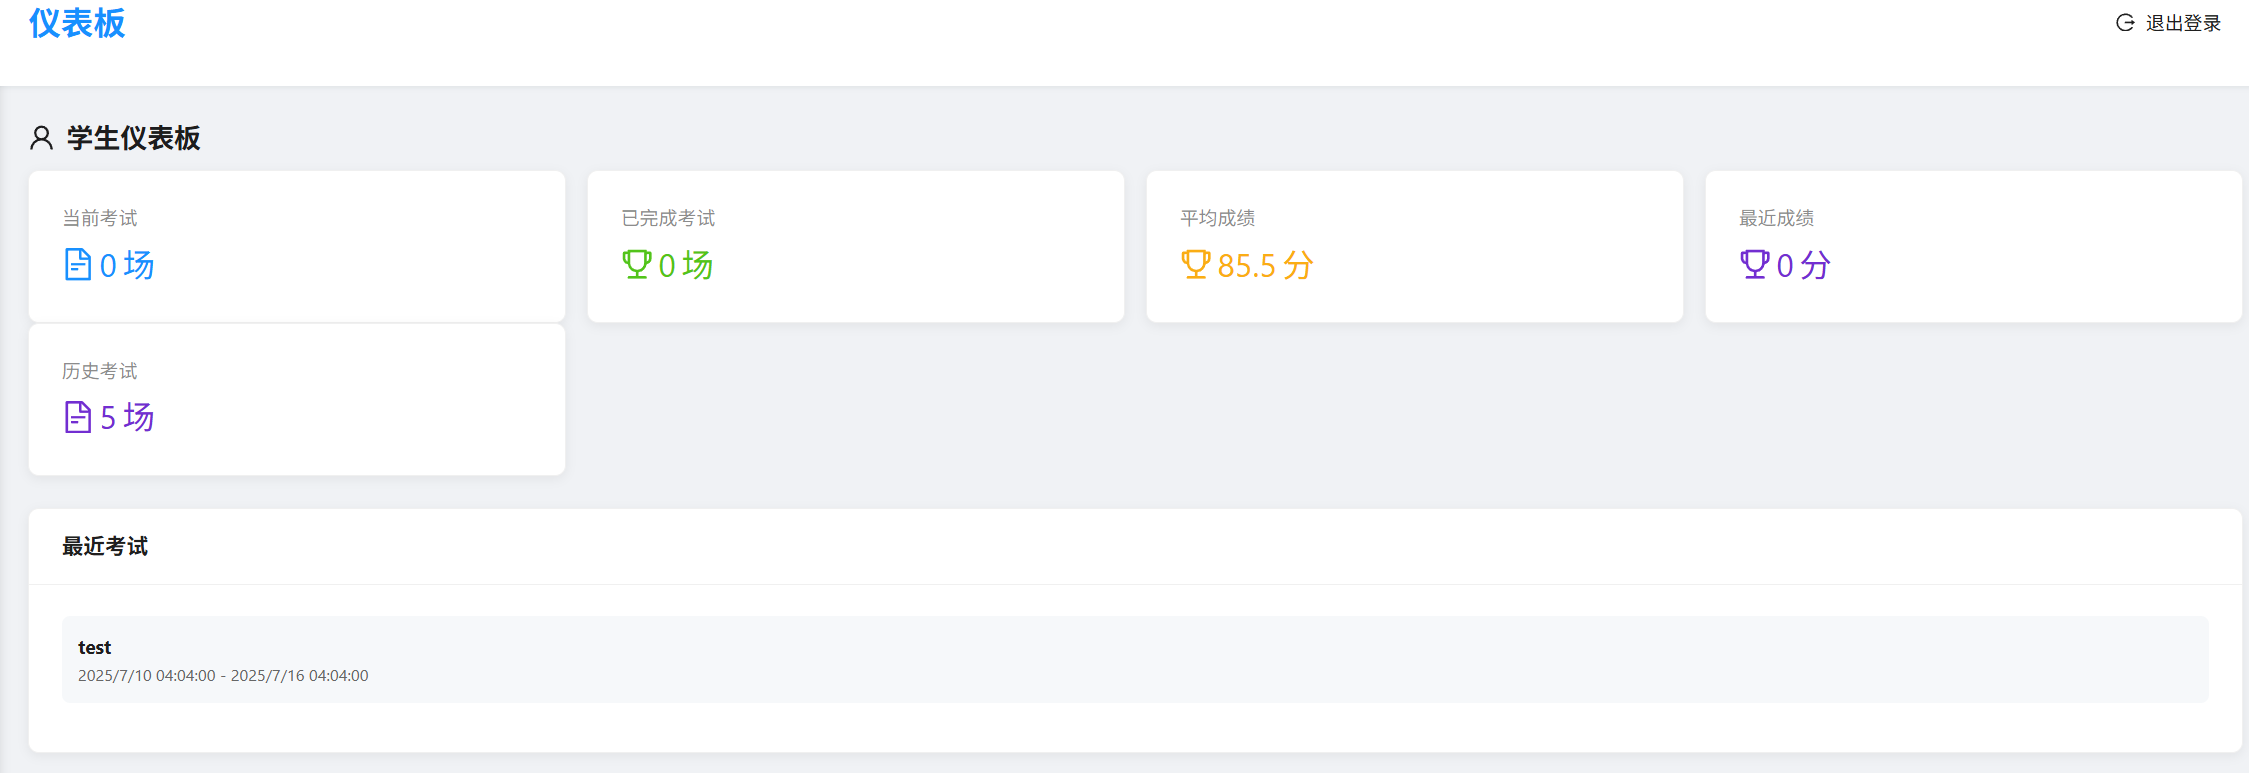
\includegraphics[width=0.8\textwidth]{student/dashboard.png}
%     \caption{Student dashboard}
%     \label{fig:StudentDashboard page}
% \end{figure}
\subsubsection{Ongoing Exams}
The ongoing exams page shows the exams that are currently in progress, and students can access the detailed information,
download files and submit their answers here.
% \begin{figure}[H]
%     \centering
%     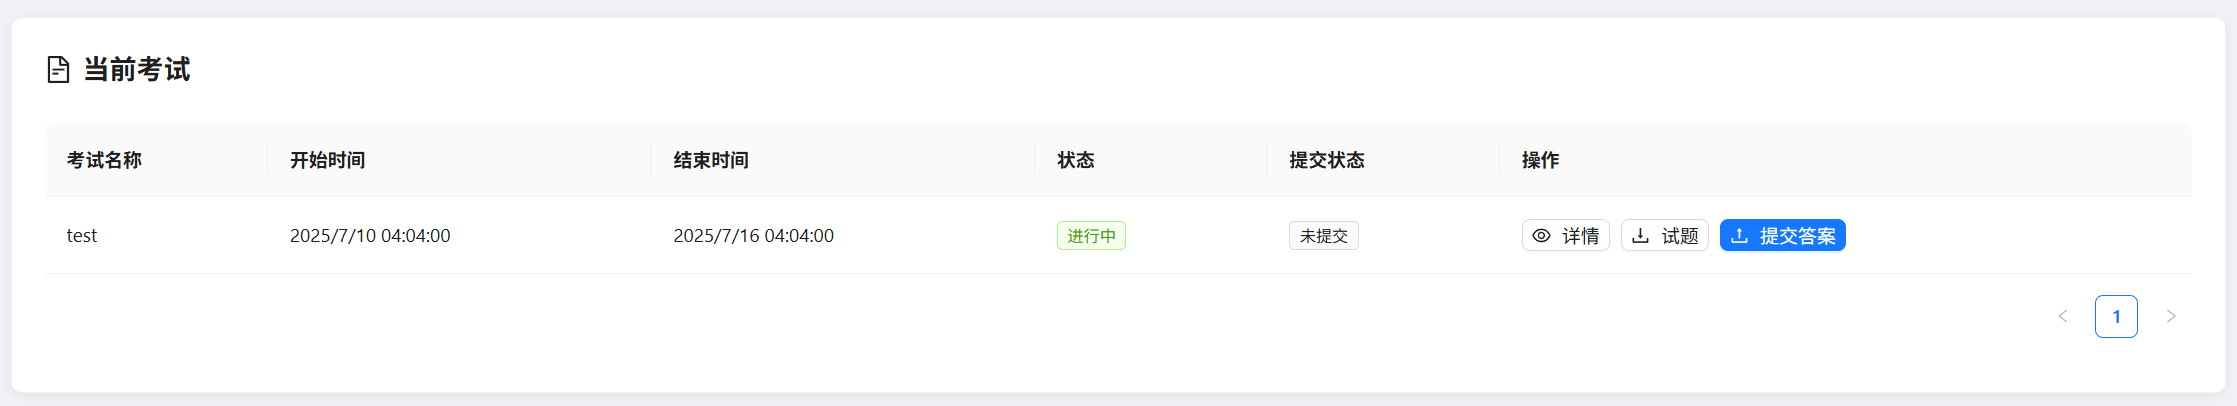
\includegraphics[width=0.8\textwidth]{student/test-ing.png}
%     \caption{Ongoing exams page}
%     \label{fig:OngoingExams page}
% \end{figure}
\subsubsection{Finished Exams}
This page shows the exams that are finished, and students can check their grades and the solutions of the exams here.
We also provide the function to download the xlsx file of the results, including the detailed grades, ranking in the region, and the overall ranking.
% \begin{figure}[H]
%     \centering
%     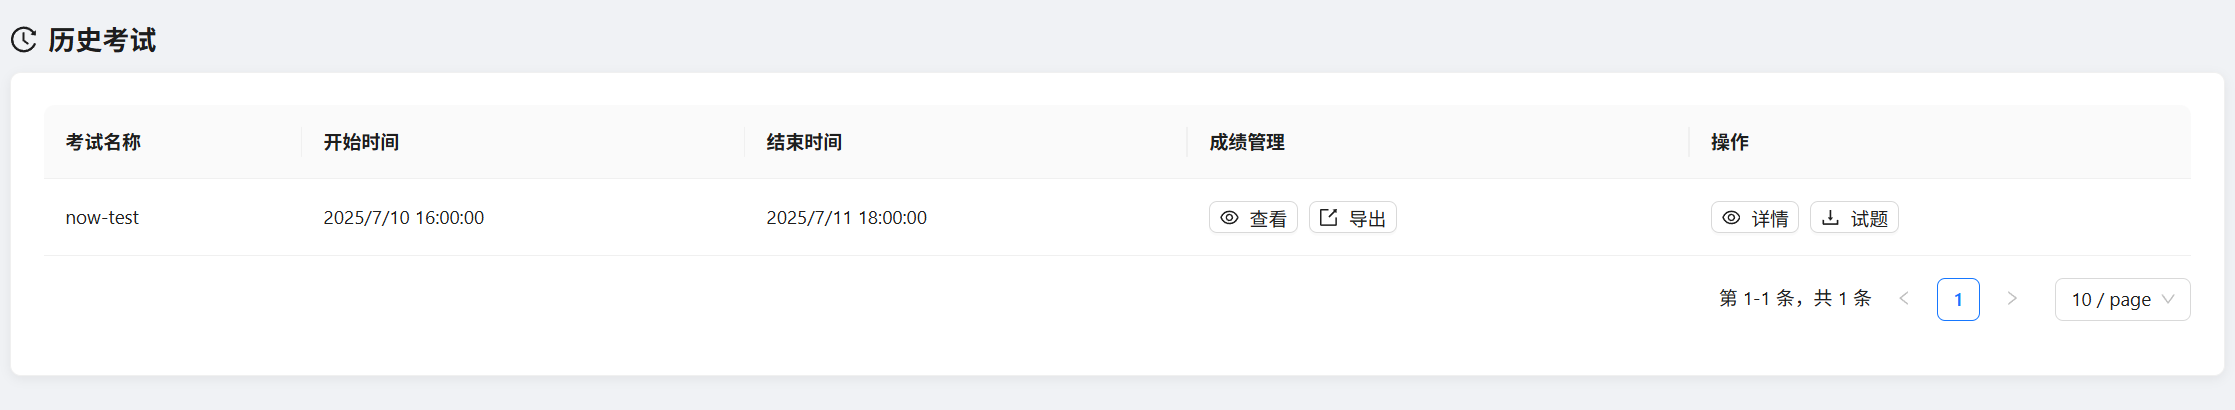
\includegraphics[width=0.8\textwidth]{student/test-his.png}
%     \caption{Finished exams page}
%     \label{fig:FinishedExams page}
% \end{figure}
\subsubsection{Account Management}
We allow students to manage their accounts, including changing their passwords, updating their avatar, and updating their username.
\subsection{Coach}
\subsubsection{Dashboard}
In the coaches' dashboard, coaches can check the information about their students, including the number of (active) students, ongoing/finished exams,
average grades and so on.
% \begin{figure}[H]
%     \centering
%     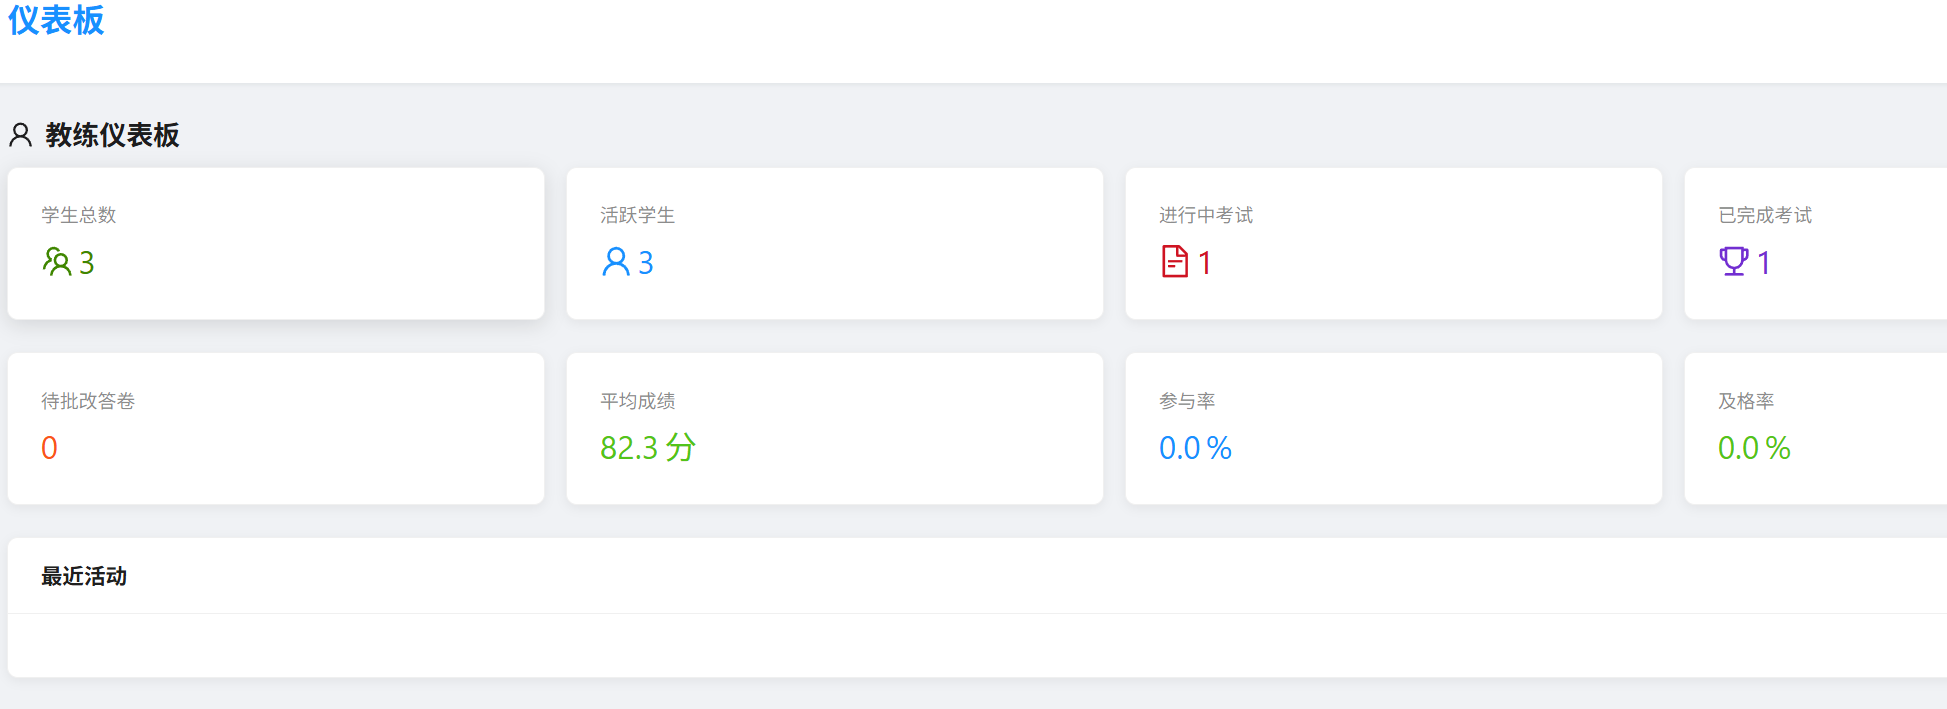
\includegraphics[width=0.7\textwidth]{coach/dashboard.png}
%     \caption{Coach dashboard}
%     \label{fig:CoachDashboard page}
% \end{figure}
\subsubsection{Student Management}
We provide the function for coaches to manage their students, including adding, deleting and editing students.
In our system, students belonging to a coach themselves have no accounts, and all their operations are done by the coach.
% insert the figure here
% \begin{figure}[H]
%     \centering
%     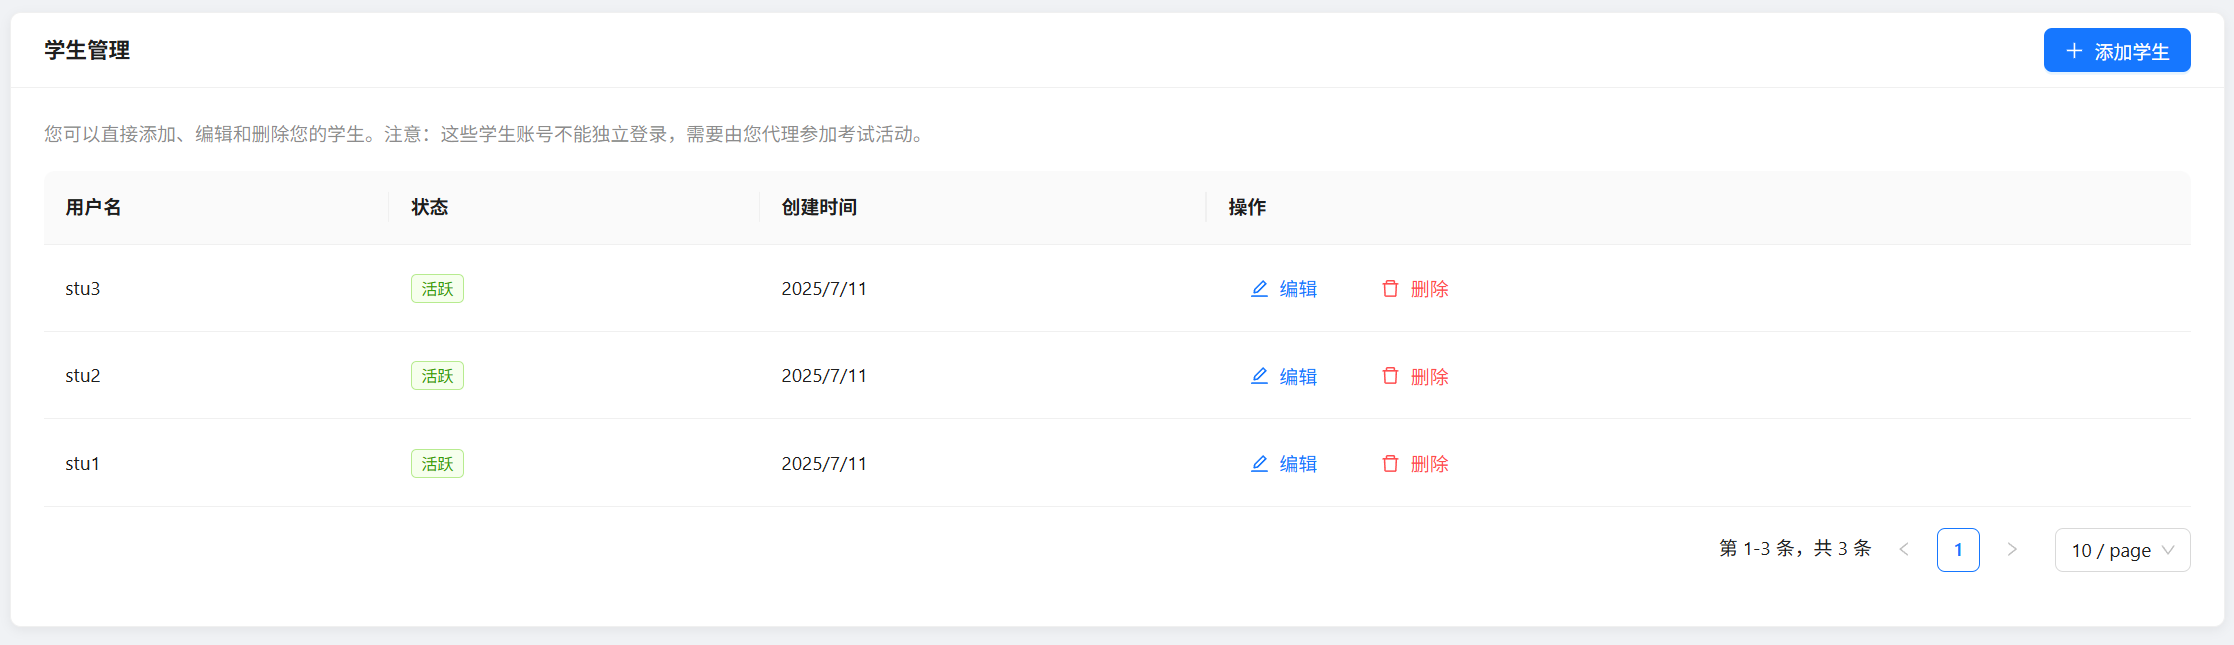
\includegraphics[width=0.7\textwidth]{coach/stu-manage.png}
%     \caption{Student management page}
%     \label{fig:StudentManagement page}
% \end{figure}
\subsubsection{Ongoing Exams}
Students belonging to a coach have no accounts, so they cannot access the exams directly, instead, coaches can access the exams
for them: the coach can download the files, and submit the answers for the students.
% \begin{figure}[H]
%     \centering
%     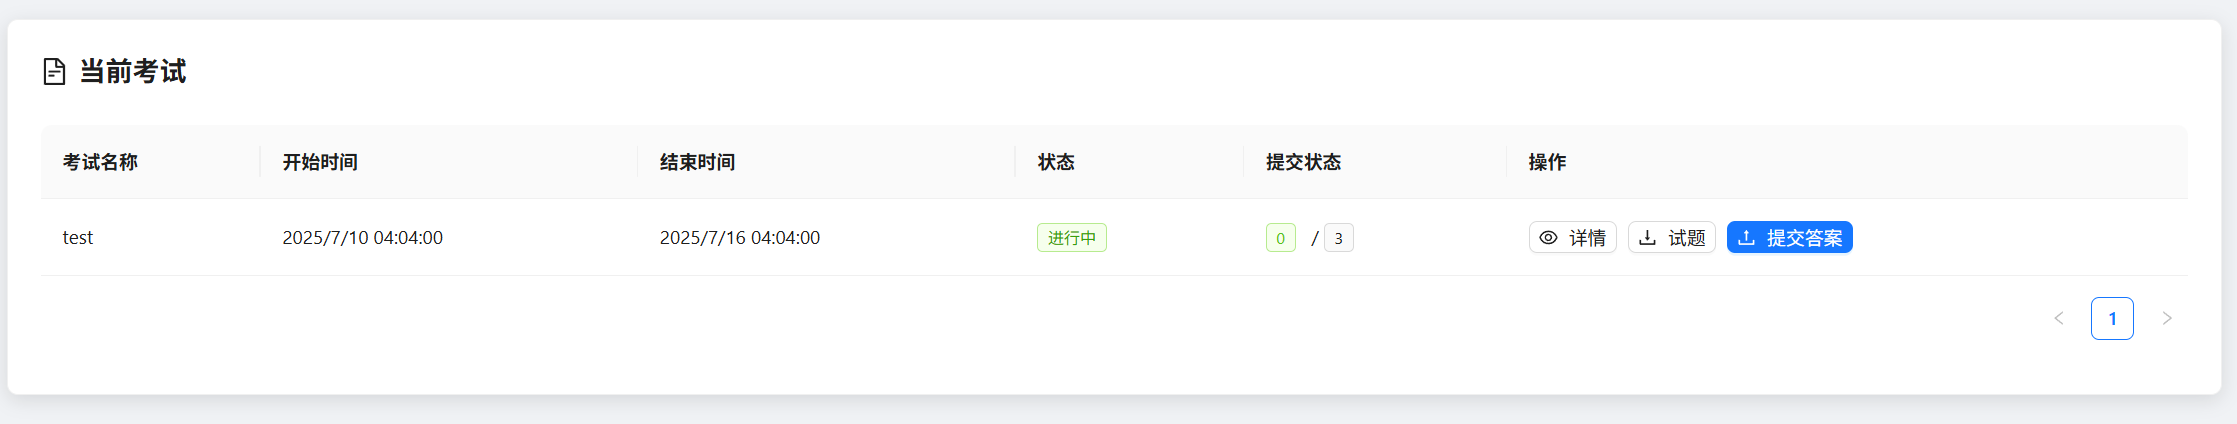
\includegraphics[width=0.8\textwidth]{coach/test-ing.png}
%     \caption{Ongoing exams page for coaches}
%     \label{fig:OngoingExamsForCoach page}
% \end{figure}
% insert the uploadexam figure here
% \begin{figure}[H]
%     \centering
%     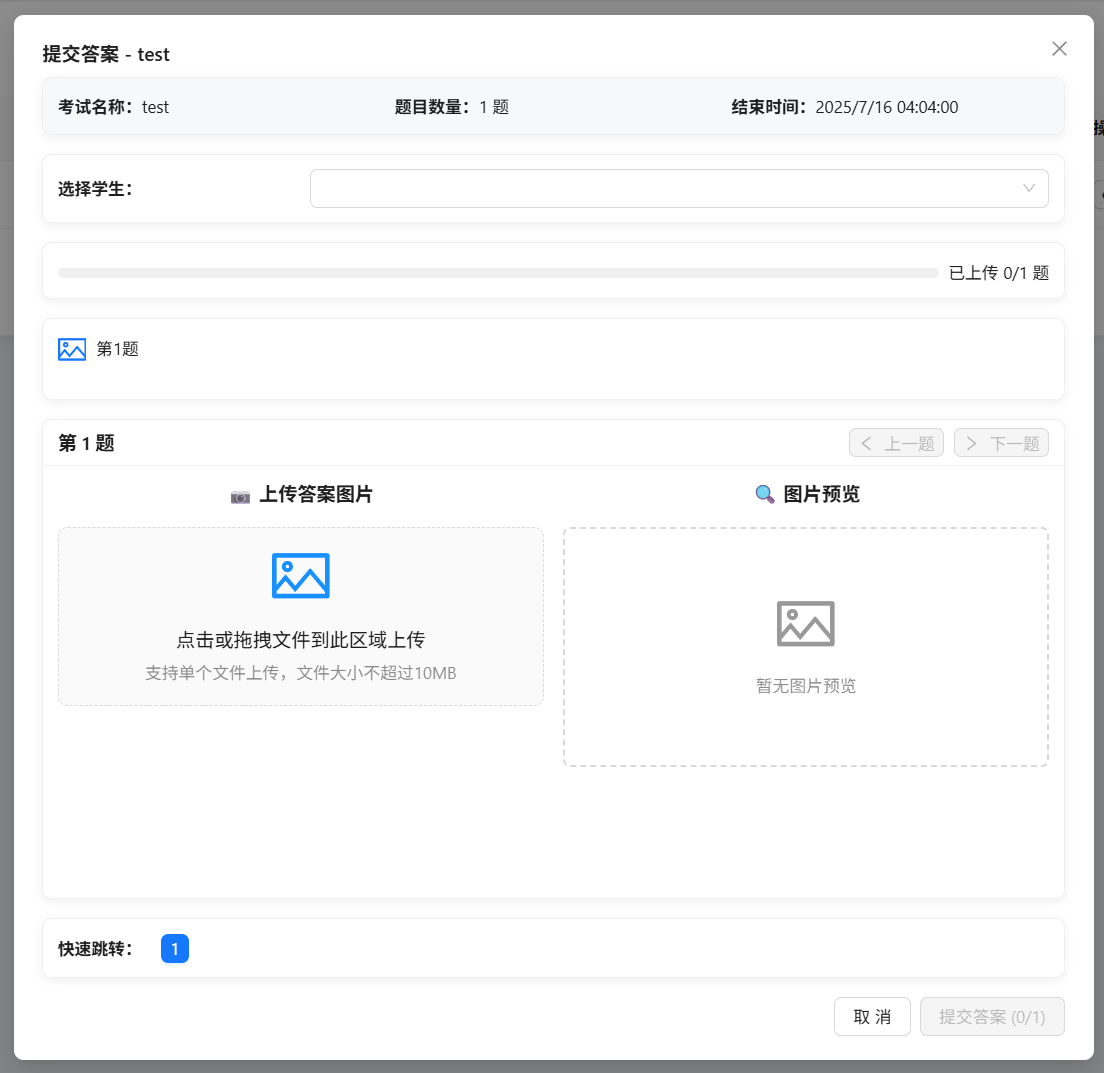
\includegraphics[width=0.4\textwidth]{coach/uploadexam.png}
%     \caption{Upload exam page for coaches}
%     \label{fig:UploadExamForCoach page}
% \end{figure}
\subsubsection{History Exams}
This page shows the finished exams of the students just like the students' finished exams page, and coaches can check the grades and solutions of the exams
for all their students.
% \begin{figure}[H]
%     \centering
%     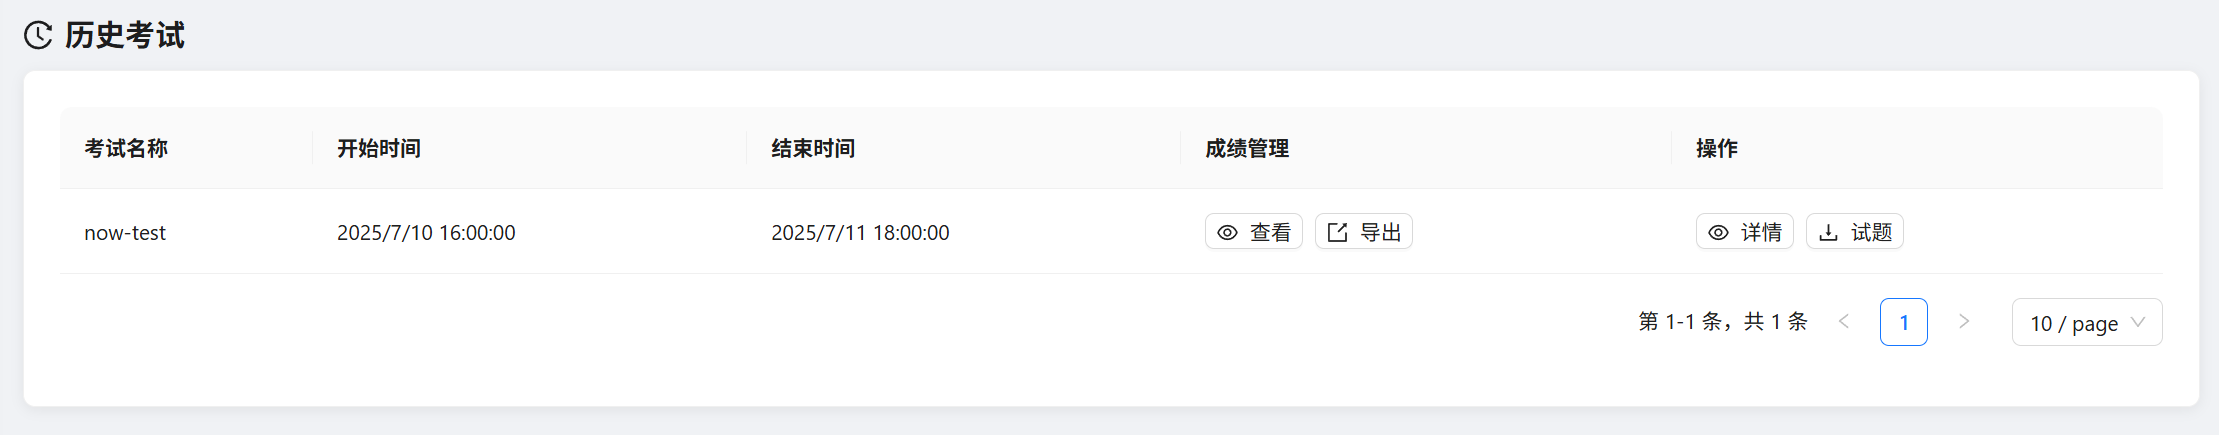
\includegraphics[width=0.8\textwidth]{coach/test-ed.png}
%     \caption{Finished exams page for coaches}
%     \label{fig:FinishedExamsForCoach page}
% \end{figure}
\subsubsection{Account Management}
We allow coaches to manage their accounts, including changing their passwords, updating their avatar, and updating their username.
% insert the figure here
\subsection{Grader}
\subsubsection{Dashboard}
In the graders' dashboard, graders can check the information about the exams they are assigned to grade, including the number of answer sheets to be graded or finished,
grading process information, and so on.
% insert the figure here
% \begin{figure}[H]
%     \centering
%     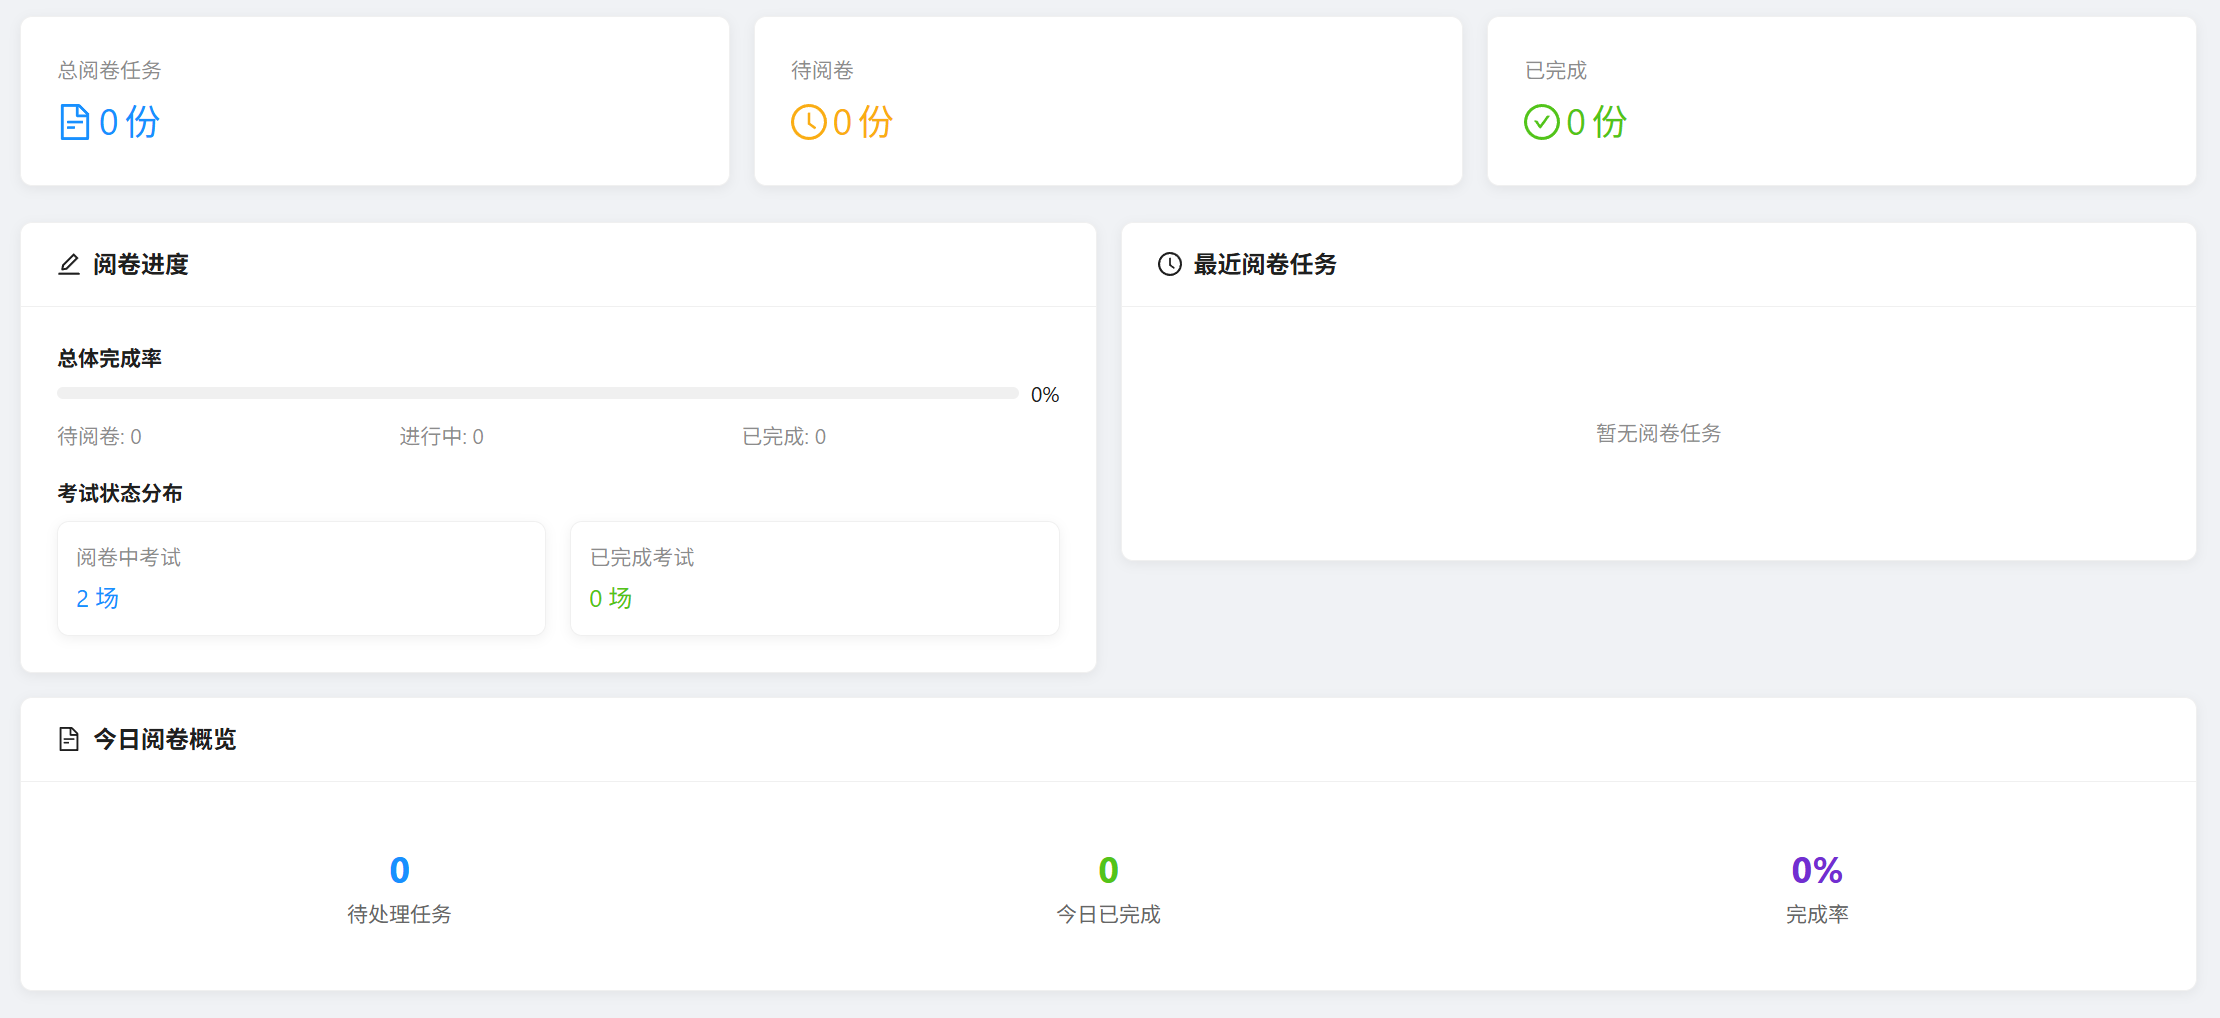
\includegraphics[width=0.8\textwidth]{grader/dashboard.png}
%     \caption{Grader dashboard}
%     \label{fig:GraderDashboard page}
% \end{figure}
\subsubsection{Grading Queue}
In the grading queue page, graders can choose the test they want to grade now and grade their assignments.
% insert the figure here
% \begin{figure}[H]
%     \centering
%     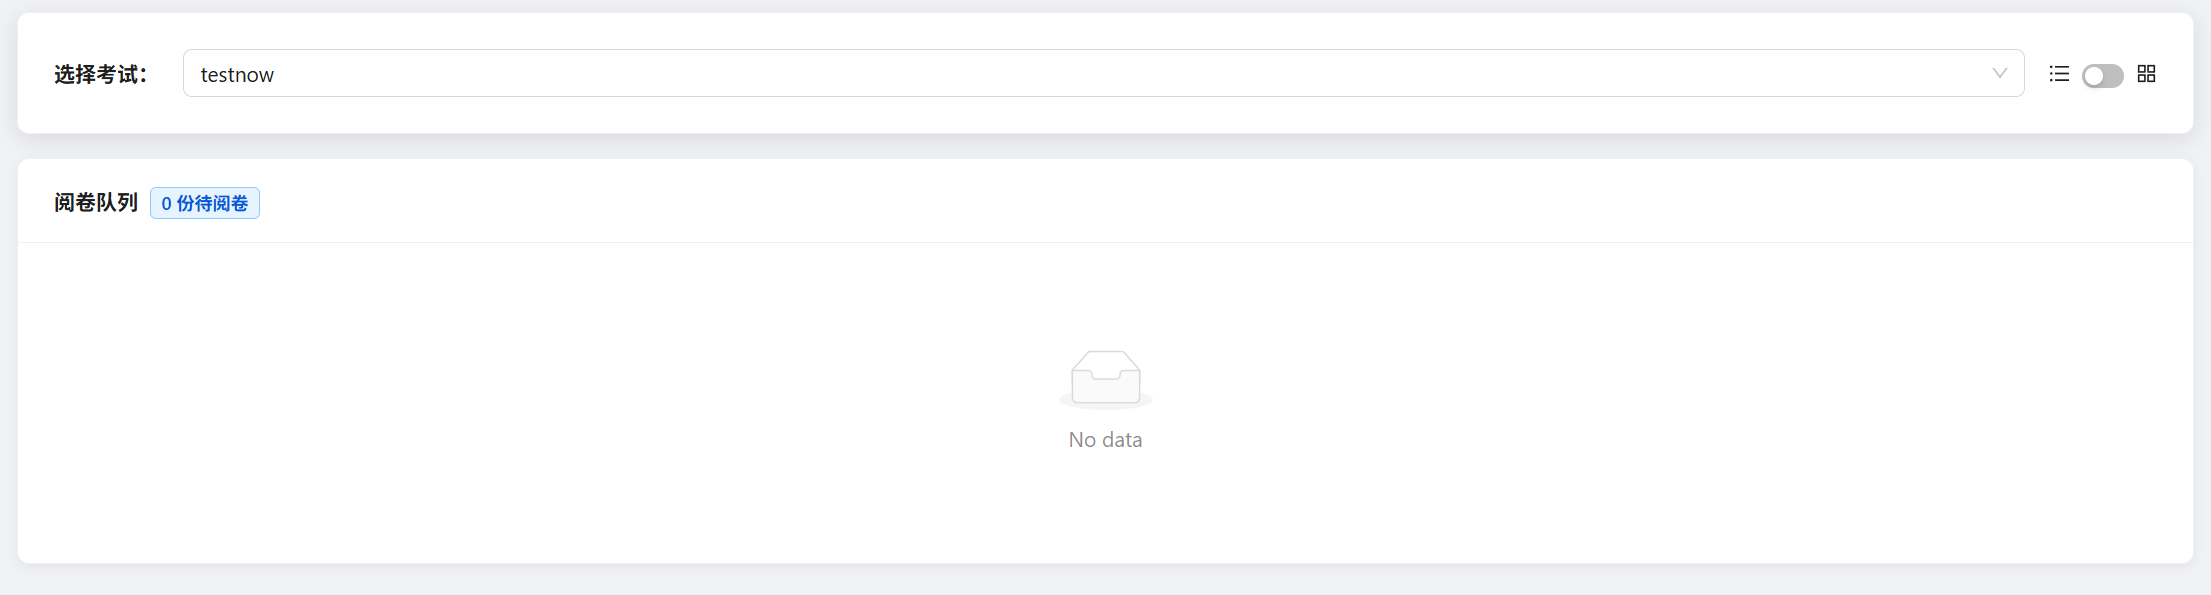
\includegraphics[width=0.8\textwidth]{grader/queue.png}
%     \caption{Grading queue page}
%     \label{fig:GradingQueue page}
% \end{figure}
\subsubsection{Account Management}
We allow graders to manage their accounts, including changing their passwords, updating their avatar, and updating their username.

\section{Summary}
% 对项目的总结和展望
\end{document}
